
\documentclass[a4paper,11pt]{article}
\usepackage[a4paper, margin=2cm]{geometry}
\usepackage{graphicx}
\usepackage{xcolor}
\usepackage{booktabs}
\usepackage{array}
\usepackage{tabularx}
\usepackage{tcolorbox}
\usepackage{enumitem}
\usepackage{tikz}
\usepackage{fancyhdr}
\usepackage{fontenc}
\usepackage{inputenc}
\usepackage{microtype}
\usepackage{parskip}
\usepackage{multirow}
\usepackage{amsmath}
\usepackage{wasysym}

\tcbuselibrary{skins, breakable}

\definecolor{headerblue}{RGB}{30,60,120}
\definecolor{optionA}{RGB}{210,228,255}
\definecolor{optionB}{RGB}{210,245,220}
\definecolor{lightgray}{RGB}{245,245,245}
\definecolor{sectiongray}{RGB}{220,230,245}
\definecolor{warnred}{RGB}{180,30,30}

\pagestyle{fancy}
\fancyhf{}
\fancyhead[L]{\small\textcolor{headerblue}{\textbf{CLARITY vs GT --- Blind Expert Evaluation}}}
\fancyhead[R]{\small\textcolor{gray}{CONFIDENTIAL}}
\fancyfoot[C]{\small\textcolor{gray}{Page \thepage\ --- Do not discuss with other reviewers}}
\renewcommand{\headrulewidth}{0.4pt}

\newcommand{\checkbox}{\Square}
\newcommand{\sectionbar}[1]{%
  \vspace{4pt}
  {\colorbox{sectiongray}{\makebox[\dimexpr\linewidth-2\fboxsep\relax][l]{\strut\textbf{\small #1}}}}\vspace{3pt}
}
\newcommand{\inforow}[2]{%
  \makebox[5cm][l]{\textbf{\small #1:}} {\small #2}\\[2pt]
}

\begin{document}

\newpage

\begin{tcolorbox}[colback=headerblue,colframe=headerblue,arc=3pt]
  \color{white}\large\bfseries
  Case 01 \hfill TP1 $\rightarrow$ TP2
\end{tcolorbox}
{\footnotesize\textit{Patient identity anonymized. Do not attempt to de-identify.}}

\sectionbar{Patient Summary}
\begin{tabular}{@{}p{5.5cm}p{10cm}@{}}
  \textbf{\small Age / Sex:} & {\small 26 / Female} \\
  \textbf{\small Race:} & {\small White} \\
  \textbf{\small Diagnosis:} & {\small ASTROCYTOMA, WHO Grade 2} \\
  \textbf{\small Days from diagnosis:} & {\small 90} \\
  \textbf{\small Disease status:} & {\small Progression documented} \\
  \textbf{\small Key molecular markers:} & {\small IDH1 WT;  IDH2 WT;  MGMT unmethylated} \\
  \textbf{\small Interval to next scan:} & {\small 24 days} \\
\end{tabular}

\sectionbar{Prior Treatment (at pre-scan timepoint)}
\begin{itemize}[leftmargin=1.5em,itemsep=0pt,topsep=2pt]
  \item \textbf{RT}: 60.0\,Gy / 30 fractions
  \item \textbf{Chemo}: Temozolomide (continuous)
  \item \textbf{Other}: avastin, everolimus (continuous)
\end{itemize}

\sectionbar{MRI at Pre-treatment Timepoint}
\begin{center}
  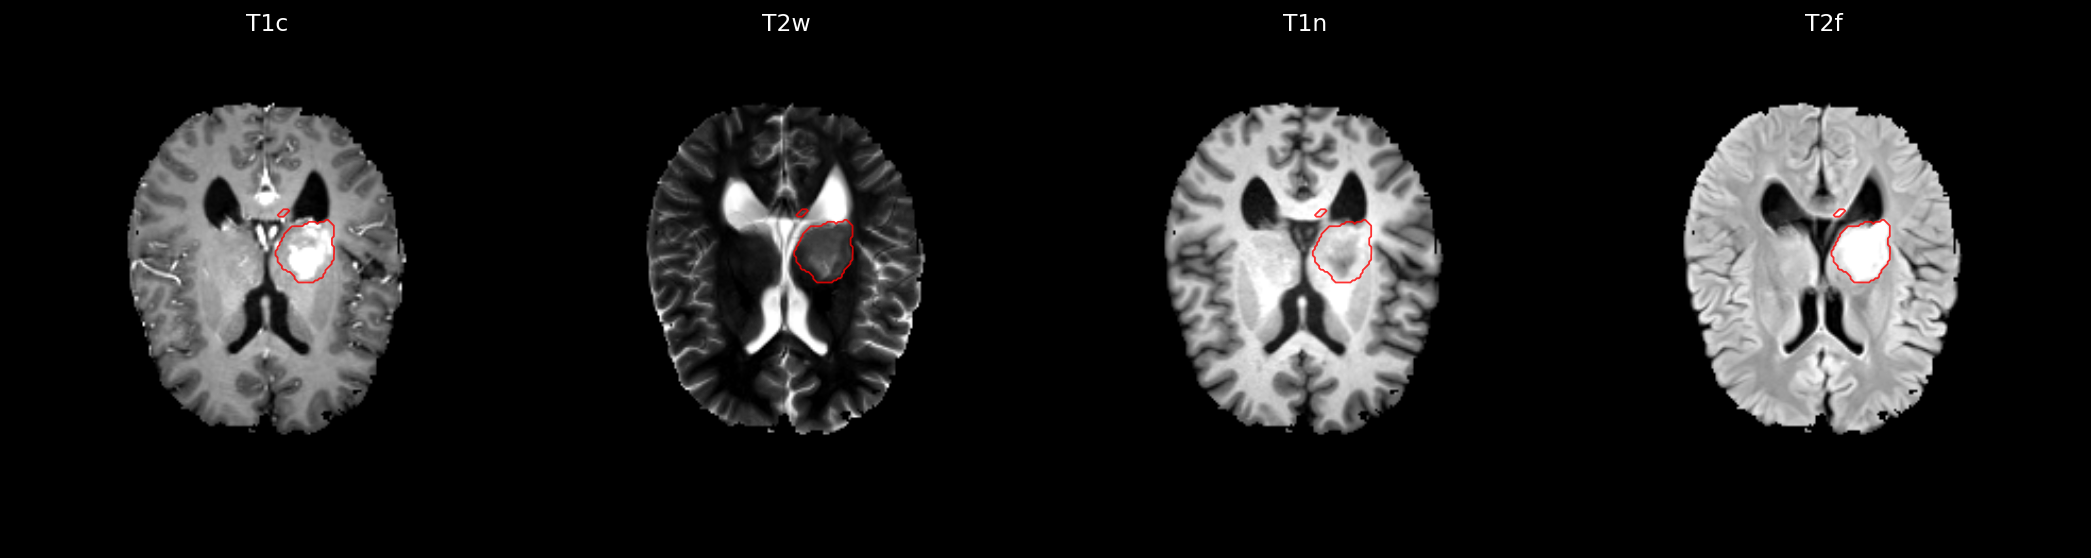
\includegraphics[width=\linewidth]{mri_slices/case_01_mri.png}
\end{center}
{\footnotesize\centering\textit{Red contour = tumor mask. Left to right: T1c, T2w, T1n, T2f (axial slice through tumor center).}\\}

\sectionbar{Proposed Treatment Plans for Next Interval}
{\footnotesize\textit{One option is the actual physician-prescribed regimen; the other is an AI-generated candidate. You do not know which is which.}}

\begin{tcolorbox}[colback=optionA,colframe=optionA!60!black,arc=3pt,title={\textbf{Treatment Option A}},fonttitle=\normalsize\bfseries]
  \begin{itemize}[leftmargin=1.5em,itemsep=1pt,topsep=0pt]
    \item \textbf{Immuno}: Avastin $\times$4 cycles (q21d)
    \item \textbf{Adjuvant}: Temozolomide $\times$4 cycles (q28d)
    \item \textbf{Other}: avastin, everolimus (continuous)
  \end{itemize}
\end{tcolorbox}

\begin{tcolorbox}[colback=optionB,colframe=optionB!60!black,arc=3pt,title={\textbf{Treatment Option B}},fonttitle=\normalsize\bfseries]
  \begin{itemize}[leftmargin=1.5em,itemsep=1pt,topsep=0pt]
    \item \textbf{Immuno}: Bevacizumab $\times$ongoing cycles (q14d)
    \item \textbf{Adjuvant}: Temozolomide $\times$6 cycles (q28d)
  \end{itemize}
\end{tcolorbox}

\sectionbar{Expert Judgment (circle or mark ONE)}
\begin{enumerate}[label=\alph*.,leftmargin=2em,itemsep=4pt,topsep=2pt]
  \item[\checkbox] \textbf{Option A} is more clinically reasonable
  \item[\checkbox] \textbf{Option B} is more clinically reasonable
  \item[\checkbox] Both options are \textbf{clinically equivalent} / acceptable
\end{enumerate}

\sectionbar{Confidence Level \normalfont\small(1 = Very uncertain \quad 5 = Very confident)}
\quad $\checkbox$~1 \qquad $\checkbox$~2 \qquad $\checkbox$~3 \qquad $\checkbox$~4 \qquad $\checkbox$~5

\sectionbar{Optional Comment}
\vspace{1.5cm}\hrule\vspace{0.8cm}\hrule

{\footnotesize\textcolor{gray}{\hfill Generated: 2026-05-08 \quad Study ID: CLARITY-BLIND-01}}
\newpage

\begin{tcolorbox}[colback=headerblue,colframe=headerblue,arc=3pt]
  \color{white}\large\bfseries
  Case 02 \hfill TP1 $\rightarrow$ TP2
\end{tcolorbox}
{\footnotesize\textit{Patient identity anonymized. Do not attempt to de-identify.}}

\sectionbar{Patient Summary}
\begin{tabular}{@{}p{5.5cm}p{10cm}@{}}
  \textbf{\small Age / Sex:} & {\small 35 / Male} \\
  \textbf{\small Race:} & {\small White} \\
  \textbf{\small Diagnosis:} & {\small DIFFUSE GLIOMA, WHO Grade 4} \\
  \textbf{\small Days from diagnosis:} & {\small 0} \\
  \textbf{\small Disease status:} & {\small Progression documented} \\
  \textbf{\small Key molecular markers:} & {\small IDH1 mut;  IDH2 WT;  TP53 alt} \\
  \textbf{\small Interval to next scan:} & {\small 136 days} \\
\end{tabular}

\sectionbar{Prior Treatment (at pre-scan timepoint)}
\begin{itemize}[leftmargin=1.5em,itemsep=0pt,topsep=2pt]
  \item \textit{Observation / No active therapy}
\end{itemize}

\sectionbar{MRI at Pre-treatment Timepoint}
\begin{center}
  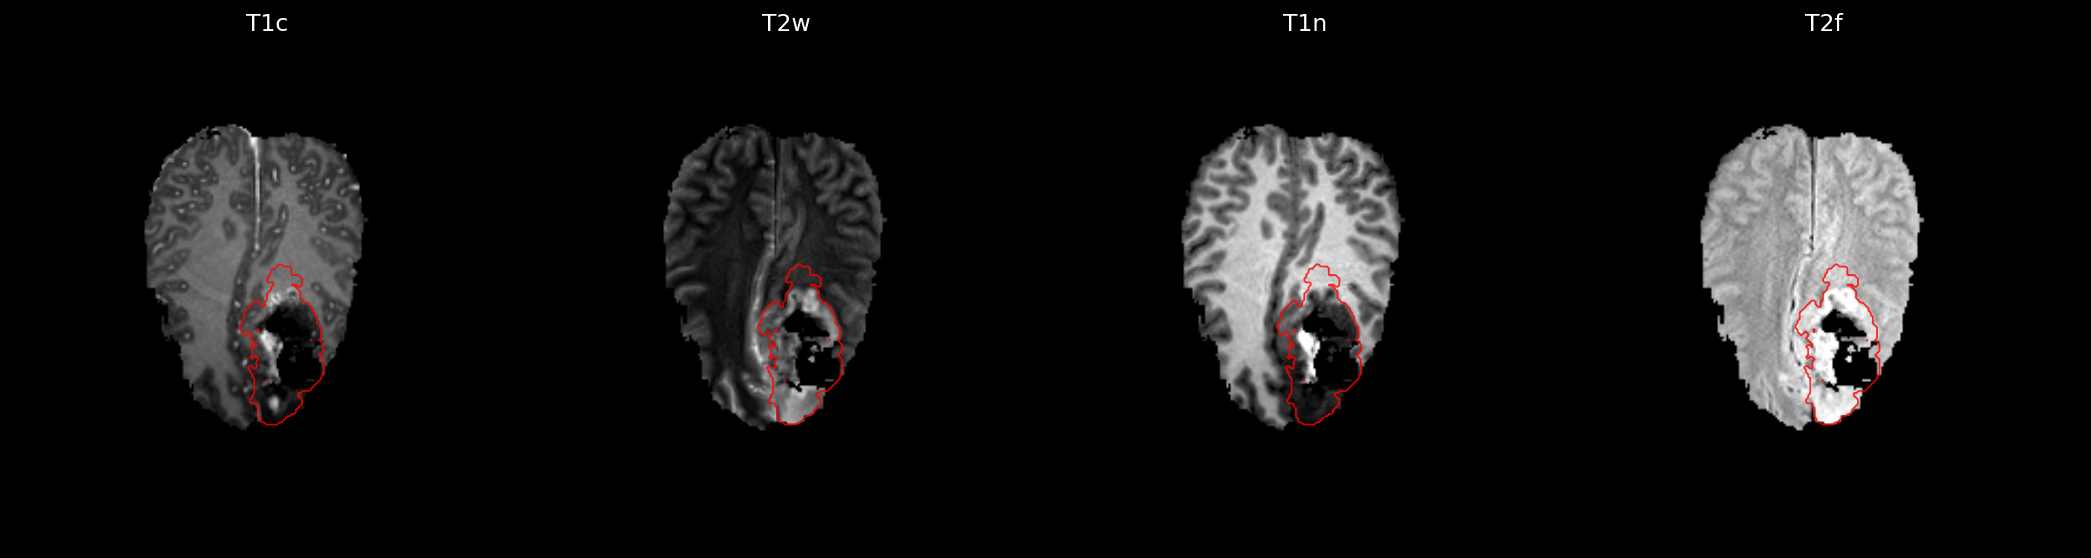
\includegraphics[width=\linewidth]{mri_slices/case_02_mri.png}
\end{center}
{\footnotesize\centering\textit{Red contour = tumor mask. Left to right: T1c, T2w, T1n, T2f (axial slice through tumor center).}\\}

\sectionbar{Proposed Treatment Plans for Next Interval}
{\footnotesize\textit{One option is the actual physician-prescribed regimen; the other is an AI-generated candidate. You do not know which is which.}}

\begin{tcolorbox}[colback=optionA,colframe=optionA!60!black,arc=3pt,title={\textbf{Treatment Option A}},fonttitle=\normalsize\bfseries]
  \begin{itemize}[leftmargin=1.5em,itemsep=1pt,topsep=0pt]
    \item \textbf{RT}: 60.0\,Gy / 30 fractions
    \item \textbf{Chemo}: Temozolomide (continuous)
  \end{itemize}
\end{tcolorbox}

\begin{tcolorbox}[colback=optionB,colframe=optionB!60!black,arc=3pt,title={\textbf{Treatment Option B}},fonttitle=\normalsize\bfseries]
  \begin{itemize}[leftmargin=1.5em,itemsep=1pt,topsep=0pt]
    \item \textbf{RT}: 60.0\,Gy / 30 fractions
    \item \textbf{Chemo}: Temozolomide (continuous)
    \item \textbf{Adjuvant}: Temozolomide $\times$6 cycles (q28d)
    \item \textbf{Other}: Optune TTF (continuous)
  \end{itemize}
\end{tcolorbox}

\sectionbar{Expert Judgment (circle or mark ONE)}
\begin{enumerate}[label=\alph*.,leftmargin=2em,itemsep=4pt,topsep=2pt]
  \item[\checkbox] \textbf{Option A} is more clinically reasonable
  \item[\checkbox] \textbf{Option B} is more clinically reasonable
  \item[\checkbox] Both options are \textbf{clinically equivalent} / acceptable
\end{enumerate}

\sectionbar{Confidence Level \normalfont\small(1 = Very uncertain \quad 5 = Very confident)}
\quad $\checkbox$~1 \qquad $\checkbox$~2 \qquad $\checkbox$~3 \qquad $\checkbox$~4 \qquad $\checkbox$~5

\sectionbar{Optional Comment}
\vspace{1.5cm}\hrule\vspace{0.8cm}\hrule

{\footnotesize\textcolor{gray}{\hfill Generated: 2026-05-08 \quad Study ID: CLARITY-BLIND-02}}
\newpage

\begin{tcolorbox}[colback=headerblue,colframe=headerblue,arc=3pt]
  \color{white}\large\bfseries
  Case 03 \hfill TP1 $\rightarrow$ TP2
\end{tcolorbox}
{\footnotesize\textit{Patient identity anonymized. Do not attempt to de-identify.}}

\sectionbar{Patient Summary}
\begin{tabular}{@{}p{5.5cm}p{10cm}@{}}
  \textbf{\small Age / Sex:} & {\small 45 / Male} \\
  \textbf{\small Race:} & {\small White} \\
  \textbf{\small Diagnosis:} & {\small DIFFUSE GLIOMA, WHO Grade 4} \\
  \textbf{\small Days from diagnosis:} & {\small 11} \\
  \textbf{\small Disease status:} & {\small Progression documented} \\
  \textbf{\small Key molecular markers:} & {\small IDH1 mut;  IDH2 WT;  MGMT methylated;  TP53 alt} \\
  \textbf{\small Interval to next scan:} & {\small 97 days} \\
\end{tabular}

\sectionbar{Prior Treatment (at pre-scan timepoint)}
\begin{itemize}[leftmargin=1.5em,itemsep=0pt,topsep=2pt]
  \item \textit{Observation / No active therapy}
\end{itemize}

\sectionbar{MRI at Pre-treatment Timepoint}
\begin{center}
  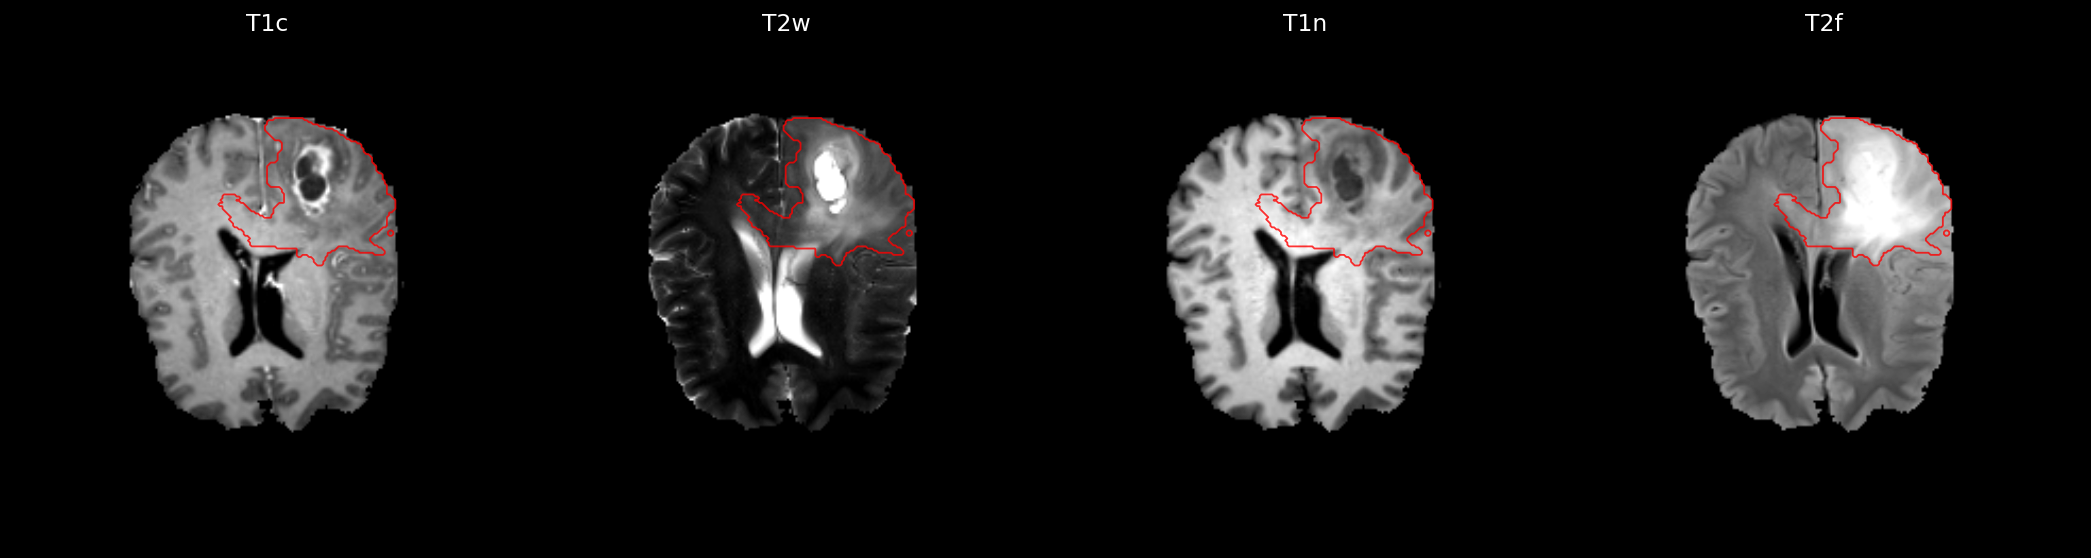
\includegraphics[width=\linewidth]{mri_slices/case_03_mri.png}
\end{center}
{\footnotesize\centering\textit{Red contour = tumor mask. Left to right: T1c, T2w, T1n, T2f (axial slice through tumor center).}\\}

\sectionbar{Proposed Treatment Plans for Next Interval}
{\footnotesize\textit{One option is the actual physician-prescribed regimen; the other is an AI-generated candidate. You do not know which is which.}}

\begin{tcolorbox}[colback=optionA,colframe=optionA!60!black,arc=3pt,title={\textbf{Treatment Option A}},fonttitle=\normalsize\bfseries]
  \begin{itemize}[leftmargin=1.5em,itemsep=1pt,topsep=0pt]
    \item \textbf{RT}: 60.0\,Gy / 30 fractions
    \item \textbf{Chemo}: Temozolomide (continuous)
    \item \textbf{Adjuvant}: Temozolomide $\times$12 cycles (q28d)
    \item \textbf{Other}: Optune TTF (continuous)
  \end{itemize}
\end{tcolorbox}

\begin{tcolorbox}[colback=optionB,colframe=optionB!60!black,arc=3pt,title={\textbf{Treatment Option B}},fonttitle=\normalsize\bfseries]
  \begin{itemize}[leftmargin=1.5em,itemsep=1pt,topsep=0pt]
    \item \textbf{RT}: 60.0\,Gy / 30 fractions
    \item \textbf{Chemo}: Temozolomide (continuous)
    \item \textbf{Adjuvant}: Temozolomide $\times$6 cycles (q28d)
  \end{itemize}
\end{tcolorbox}

\sectionbar{Expert Judgment (circle or mark ONE)}
\begin{enumerate}[label=\alph*.,leftmargin=2em,itemsep=4pt,topsep=2pt]
  \item[\checkbox] \textbf{Option A} is more clinically reasonable
  \item[\checkbox] \textbf{Option B} is more clinically reasonable
  \item[\checkbox] Both options are \textbf{clinically equivalent} / acceptable
\end{enumerate}

\sectionbar{Confidence Level \normalfont\small(1 = Very uncertain \quad 5 = Very confident)}
\quad $\checkbox$~1 \qquad $\checkbox$~2 \qquad $\checkbox$~3 \qquad $\checkbox$~4 \qquad $\checkbox$~5

\sectionbar{Optional Comment}
\vspace{1.5cm}\hrule\vspace{0.8cm}\hrule

{\footnotesize\textcolor{gray}{\hfill Generated: 2026-05-08 \quad Study ID: CLARITY-BLIND-03}}
\newpage

\begin{tcolorbox}[colback=headerblue,colframe=headerblue,arc=3pt]
  \color{white}\large\bfseries
  Case 04 \hfill TP1 $\rightarrow$ TP2
\end{tcolorbox}
{\footnotesize\textit{Patient identity anonymized. Do not attempt to de-identify.}}

\sectionbar{Patient Summary}
\begin{tabular}{@{}p{5.5cm}p{10cm}@{}}
  \textbf{\small Age / Sex:} & {\small 63 / Female} \\
  \textbf{\small Race:} & {\small White} \\
  \textbf{\small Diagnosis:} & {\small ASTROCYTOMA, WHO Grade 3} \\
  \textbf{\small Days from diagnosis:} & {\small 19} \\
  \textbf{\small Disease status:} & {\small Progression documented} \\
  \textbf{\small Key molecular markers:} & {\small IDH1 WT;  IDH2 WT;  MGMT methylated} \\
  \textbf{\small Interval to next scan:} & {\small 26 days} \\
\end{tabular}

\sectionbar{Prior Treatment (at pre-scan timepoint)}
\begin{itemize}[leftmargin=1.5em,itemsep=0pt,topsep=2pt]
  \item \textit{Observation / No active therapy}
\end{itemize}

\sectionbar{MRI at Pre-treatment Timepoint}
\begin{center}
  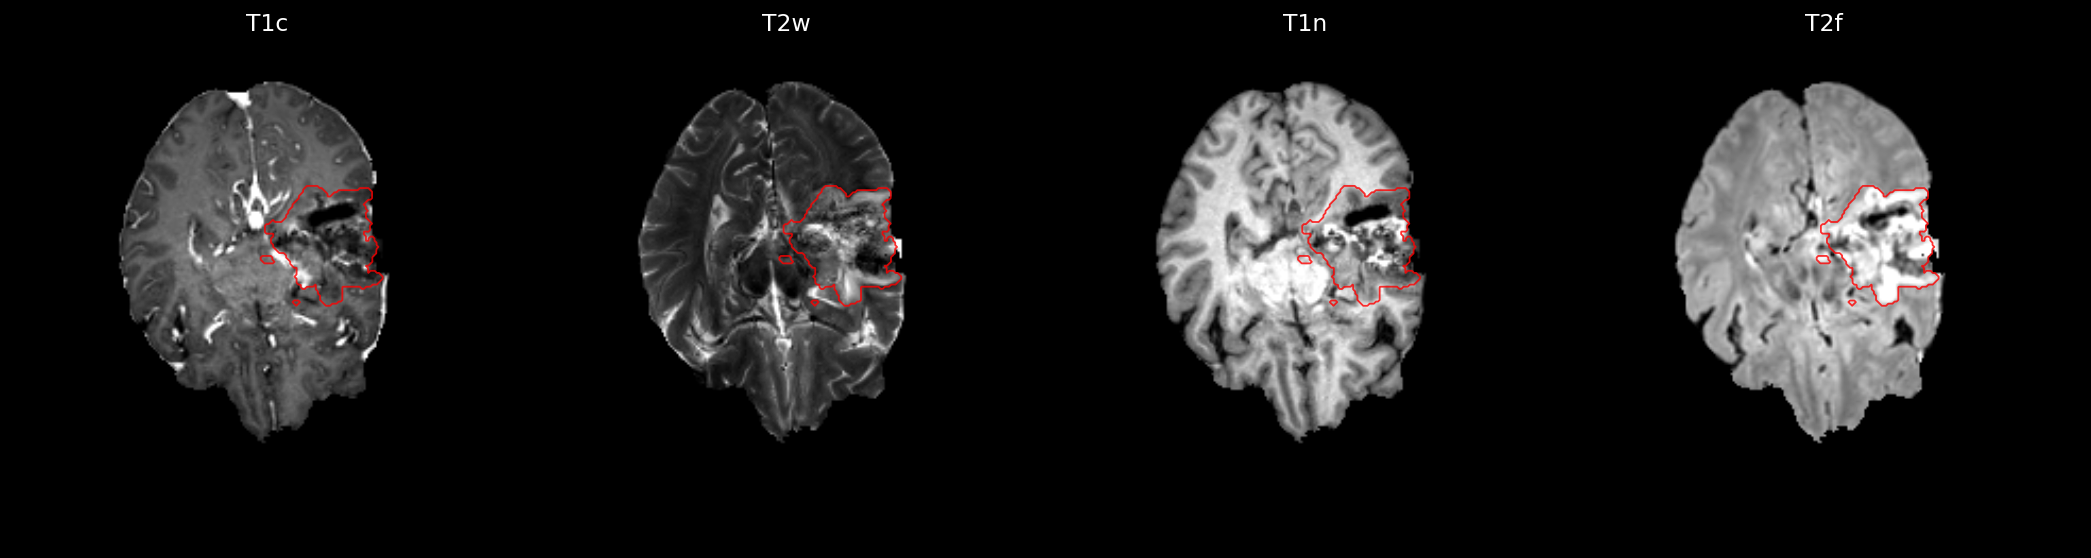
\includegraphics[width=\linewidth]{mri_slices/case_04_mri.png}
\end{center}
{\footnotesize\centering\textit{Red contour = tumor mask. Left to right: T1c, T2w, T1n, T2f (axial slice through tumor center).}\\}

\sectionbar{Proposed Treatment Plans for Next Interval}
{\footnotesize\textit{One option is the actual physician-prescribed regimen; the other is an AI-generated candidate. You do not know which is which.}}

\begin{tcolorbox}[colback=optionA,colframe=optionA!60!black,arc=3pt,title={\textbf{Treatment Option A}},fonttitle=\normalsize\bfseries]
  \begin{itemize}[leftmargin=1.5em,itemsep=1pt,topsep=0pt]
    \item \textbf{RT}: 59.4\,Gy / 33 fractions
    \item \textbf{Chemo}: Temozolomide (continuous)
    \item \textbf{Adjuvant}: Temozolomide $\times$12 cycles (q28d)
  \end{itemize}
\end{tcolorbox}

\begin{tcolorbox}[colback=optionB,colframe=optionB!60!black,arc=3pt,title={\textbf{Treatment Option B}},fonttitle=\normalsize\bfseries]
  \begin{itemize}[leftmargin=1.5em,itemsep=1pt,topsep=0pt]
    \item \textbf{RT}: ?\,Gy / ? fractions
    \item \textbf{Chemo}: Temozolomide (continuous)
  \end{itemize}
\end{tcolorbox}

\sectionbar{Expert Judgment (circle or mark ONE)}
\begin{enumerate}[label=\alph*.,leftmargin=2em,itemsep=4pt,topsep=2pt]
  \item[\checkbox] \textbf{Option A} is more clinically reasonable
  \item[\checkbox] \textbf{Option B} is more clinically reasonable
  \item[\checkbox] Both options are \textbf{clinically equivalent} / acceptable
\end{enumerate}

\sectionbar{Confidence Level \normalfont\small(1 = Very uncertain \quad 5 = Very confident)}
\quad $\checkbox$~1 \qquad $\checkbox$~2 \qquad $\checkbox$~3 \qquad $\checkbox$~4 \qquad $\checkbox$~5

\sectionbar{Optional Comment}
\vspace{1.5cm}\hrule\vspace{0.8cm}\hrule

{\footnotesize\textcolor{gray}{\hfill Generated: 2026-05-08 \quad Study ID: CLARITY-BLIND-04}}
\newpage

\begin{tcolorbox}[colback=headerblue,colframe=headerblue,arc=3pt]
  \color{white}\large\bfseries
  Case 05 \hfill TP1 $\rightarrow$ TP3
\end{tcolorbox}
{\footnotesize\textit{Patient identity anonymized. Do not attempt to de-identify.}}

\sectionbar{Patient Summary}
\begin{tabular}{@{}p{5.5cm}p{10cm}@{}}
  \textbf{\small Age / Sex:} & {\small 28 / Female} \\
  \textbf{\small Race:} & {\small White} \\
  \textbf{\small Diagnosis:} & {\small OLIGODENDRO-GLIOMA, WHO Grade 2} \\
  \textbf{\small Days from diagnosis:} & {\small 105} \\
  \textbf{\small Disease status:} & {\small Progression documented} \\
  \textbf{\small Key molecular markers:} & {\small MGMT methylated;  1p/19q codeleted} \\
  \textbf{\small Interval to next scan:} & {\small 245 days} \\
\end{tabular}

\sectionbar{Prior Treatment (at pre-scan timepoint)}
\begin{itemize}[leftmargin=1.5em,itemsep=0pt,topsep=2pt]
  \item \textbf{RT}: 54.0\,Gy / 30 fractions
  \item \textbf{Adjuvant}: PCV $\times$6 cycles (q42d)
\end{itemize}

\sectionbar{MRI at Pre-treatment Timepoint}
\begin{center}
  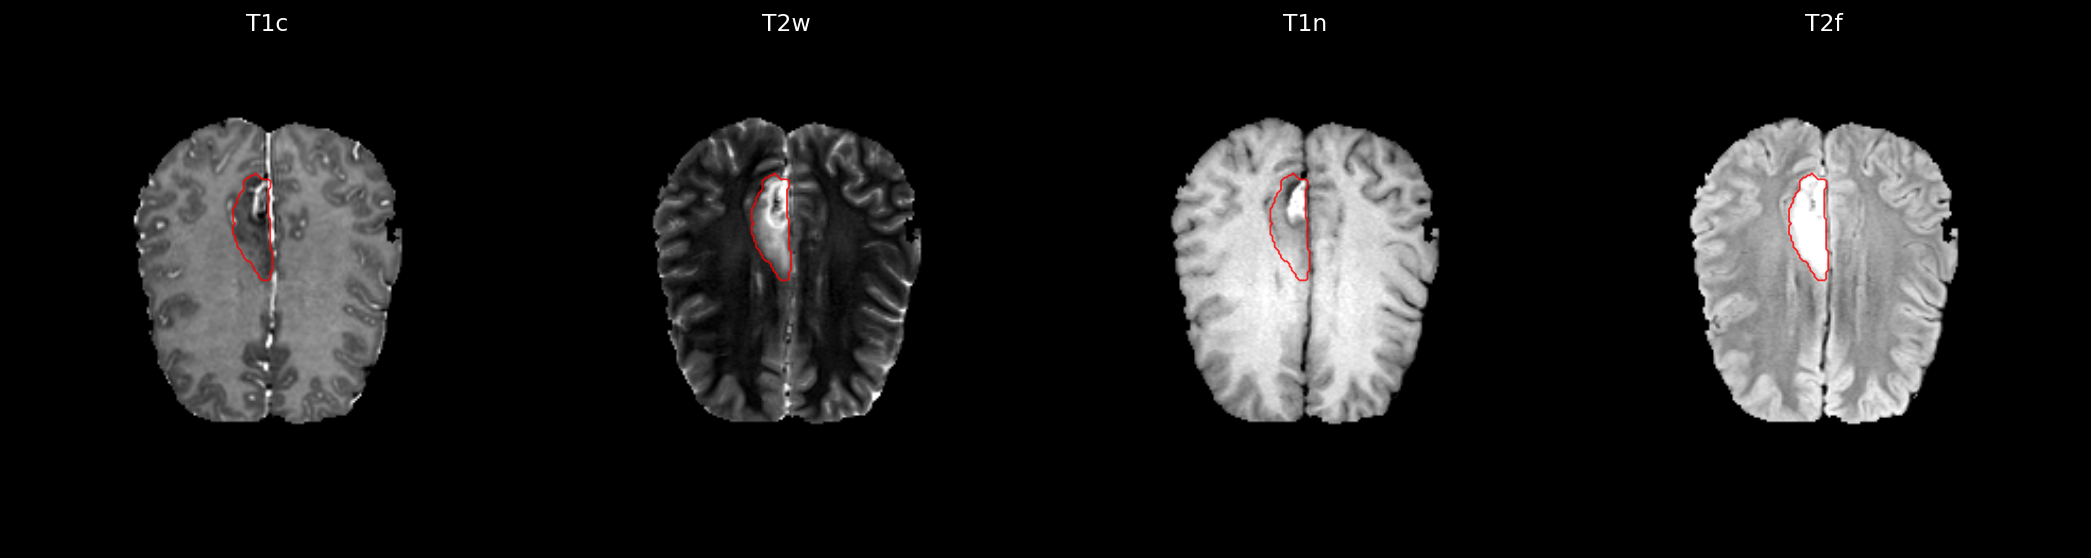
\includegraphics[width=\linewidth]{mri_slices/case_05_mri.png}
\end{center}
{\footnotesize\centering\textit{Red contour = tumor mask. Left to right: T1c, T2w, T1n, T2f (axial slice through tumor center).}\\}

\sectionbar{Proposed Treatment Plans for Next Interval}
{\footnotesize\textit{One option is the actual physician-prescribed regimen; the other is an AI-generated candidate. You do not know which is which.}}

\begin{tcolorbox}[colback=optionA,colframe=optionA!60!black,arc=3pt,title={\textbf{Treatment Option A}},fonttitle=\normalsize\bfseries]
  \begin{itemize}[leftmargin=1.5em,itemsep=1pt,topsep=0pt]
    \item \textbf{Adjuvant}: PCV $\times$6 cycles (q42d)
  \end{itemize}
\end{tcolorbox}

\begin{tcolorbox}[colback=optionB,colframe=optionB!60!black,arc=3pt,title={\textbf{Treatment Option B}},fonttitle=\normalsize\bfseries]
  \begin{itemize}[leftmargin=1.5em,itemsep=1pt,topsep=0pt]
    \item \textbf{Adjuvant}: PCV $\times$6 cycles (q42d)
  \end{itemize}
\end{tcolorbox}

\sectionbar{Expert Judgment (circle or mark ONE)}
\begin{enumerate}[label=\alph*.,leftmargin=2em,itemsep=4pt,topsep=2pt]
  \item[\checkbox] \textbf{Option A} is more clinically reasonable
  \item[\checkbox] \textbf{Option B} is more clinically reasonable
  \item[\checkbox] Both options are \textbf{clinically equivalent} / acceptable
\end{enumerate}

\sectionbar{Confidence Level \normalfont\small(1 = Very uncertain \quad 5 = Very confident)}
\quad $\checkbox$~1 \qquad $\checkbox$~2 \qquad $\checkbox$~3 \qquad $\checkbox$~4 \qquad $\checkbox$~5

\sectionbar{Optional Comment}
\vspace{1.5cm}\hrule\vspace{0.8cm}\hrule

{\footnotesize\textcolor{gray}{\hfill Generated: 2026-05-08 \quad Study ID: CLARITY-BLIND-05}}
\newpage

\begin{tcolorbox}[colback=headerblue,colframe=headerblue,arc=3pt]
  \color{white}\large\bfseries
  Case 06 \hfill TP1 $\rightarrow$ TP2
\end{tcolorbox}
{\footnotesize\textit{Patient identity anonymized. Do not attempt to de-identify.}}

\sectionbar{Patient Summary}
\begin{tabular}{@{}p{5.5cm}p{10cm}@{}}
  \textbf{\small Age / Sex:} & {\small 55 / Female} \\
  \textbf{\small Race:} & {\small White} \\
  \textbf{\small Diagnosis:} & {\small GBM, WHO Grade 4} \\
  \textbf{\small Days from diagnosis:} & {\small 78} \\
  \textbf{\small Disease status:} & {\small Progression documented} \\
  \textbf{\small Key molecular markers:} & {\small IDH1 WT;  IDH2 WT} \\
  \textbf{\small Interval to next scan:} & {\small 78 days} \\
\end{tabular}

\sectionbar{Prior Treatment (at pre-scan timepoint)}
\begin{itemize}[leftmargin=1.5em,itemsep=0pt,topsep=2pt]
  \item \textbf{RT}: ?\,Gy / ? fractions
  \item \textbf{Chemo}: Temozolomide (continuous)
\end{itemize}

\sectionbar{MRI at Pre-treatment Timepoint}
\begin{center}
  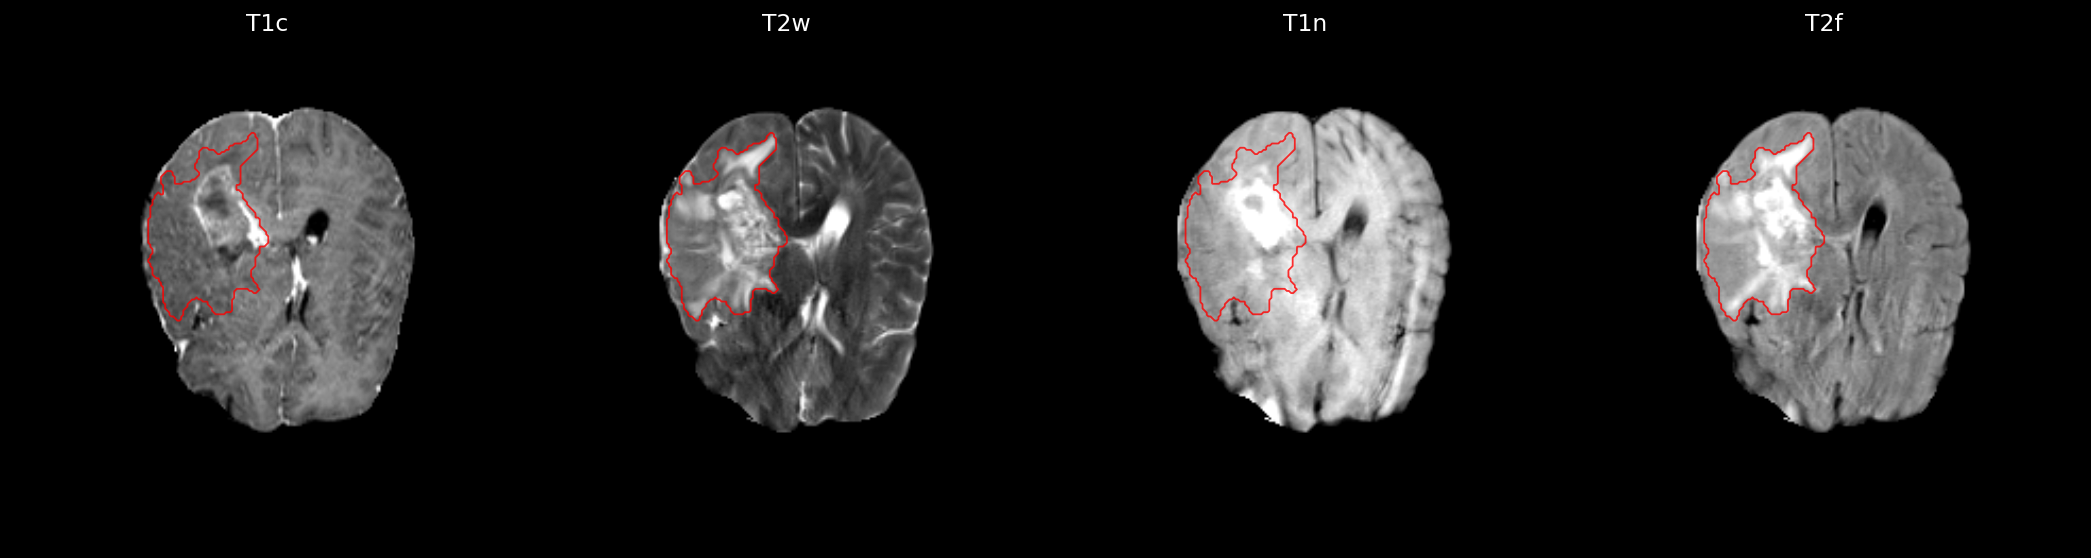
\includegraphics[width=\linewidth]{mri_slices/case_06_mri.png}
\end{center}
{\footnotesize\centering\textit{Red contour = tumor mask. Left to right: T1c, T2w, T1n, T2f (axial slice through tumor center).}\\}

\sectionbar{Proposed Treatment Plans for Next Interval}
{\footnotesize\textit{One option is the actual physician-prescribed regimen; the other is an AI-generated candidate. You do not know which is which.}}

\begin{tcolorbox}[colback=optionA,colframe=optionA!60!black,arc=3pt,title={\textbf{Treatment Option A}},fonttitle=\normalsize\bfseries]
  \begin{itemize}[leftmargin=1.5em,itemsep=1pt,topsep=0pt]
    \item \textbf{Adjuvant}: Temozolomide $\times$2 cycles (q28d)
    \item \textbf{Other}: optune ttf (continuous)
  \end{itemize}
\end{tcolorbox}

\begin{tcolorbox}[colback=optionB,colframe=optionB!60!black,arc=3pt,title={\textbf{Treatment Option B}},fonttitle=\normalsize\bfseries]
  \begin{itemize}[leftmargin=1.5em,itemsep=1pt,topsep=0pt]
    \item \textbf{Adjuvant}: Temozolomide $\times$6 cycles (q28d)
    \item \textbf{Other}: Optune TTF (continuous)
  \end{itemize}
\end{tcolorbox}

\sectionbar{Expert Judgment (circle or mark ONE)}
\begin{enumerate}[label=\alph*.,leftmargin=2em,itemsep=4pt,topsep=2pt]
  \item[\checkbox] \textbf{Option A} is more clinically reasonable
  \item[\checkbox] \textbf{Option B} is more clinically reasonable
  \item[\checkbox] Both options are \textbf{clinically equivalent} / acceptable
\end{enumerate}

\sectionbar{Confidence Level \normalfont\small(1 = Very uncertain \quad 5 = Very confident)}
\quad $\checkbox$~1 \qquad $\checkbox$~2 \qquad $\checkbox$~3 \qquad $\checkbox$~4 \qquad $\checkbox$~5

\sectionbar{Optional Comment}
\vspace{1.5cm}\hrule\vspace{0.8cm}\hrule

{\footnotesize\textcolor{gray}{\hfill Generated: 2026-05-08 \quad Study ID: CLARITY-BLIND-06}}
\newpage

\begin{tcolorbox}[colback=headerblue,colframe=headerblue,arc=3pt]
  \color{white}\large\bfseries
  Case 07 \hfill TP1 $\rightarrow$ TP3
\end{tcolorbox}
{\footnotesize\textit{Patient identity anonymized. Do not attempt to de-identify.}}

\sectionbar{Patient Summary}
\begin{tabular}{@{}p{5.5cm}p{10cm}@{}}
  \textbf{\small Age / Sex:} & {\small 25 / Male} \\
  \textbf{\small Race:} & {\small White} \\
  \textbf{\small Diagnosis:} & {\small ASTROCYTOMA, WHO Grade 2} \\
  \textbf{\small Days from diagnosis:} & {\small 105} \\
  \textbf{\small Disease status:} & {\small Progression documented} \\
  \textbf{\small Key molecular markers:} & {\small \textit{Not fully characterized}} \\
  \textbf{\small Interval to next scan:} & {\small 126 days} \\
\end{tabular}

\sectionbar{Prior Treatment (at pre-scan timepoint)}
\begin{itemize}[leftmargin=1.5em,itemsep=0pt,topsep=2pt]
  \item \textit{Observation / No active therapy}
\end{itemize}

\sectionbar{MRI at Pre-treatment Timepoint}
\begin{center}
  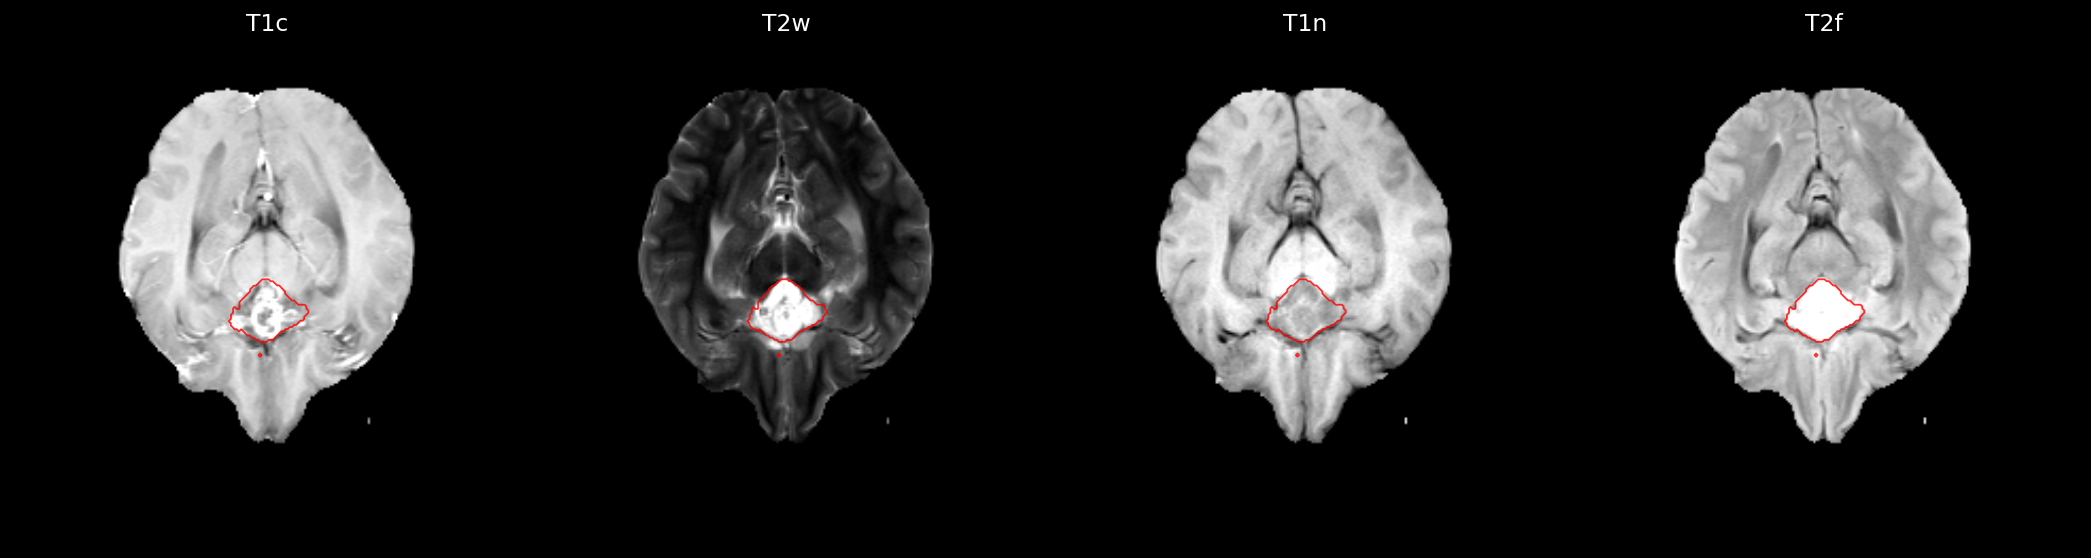
\includegraphics[width=\linewidth]{mri_slices/case_07_mri.png}
\end{center}
{\footnotesize\centering\textit{Red contour = tumor mask. Left to right: T1c, T2w, T1n, T2f (axial slice through tumor center).}\\}

\sectionbar{Proposed Treatment Plans for Next Interval}
{\footnotesize\textit{One option is the actual physician-prescribed regimen; the other is an AI-generated candidate. You do not know which is which.}}

\begin{tcolorbox}[colback=optionA,colframe=optionA!60!black,arc=3pt,title={\textbf{Treatment Option A}},fonttitle=\normalsize\bfseries]
  \begin{itemize}[leftmargin=1.5em,itemsep=1pt,topsep=0pt]
    \item \textbf{RT}: 50.4\,Gy / 28 fractions
  \end{itemize}
\end{tcolorbox}

\begin{tcolorbox}[colback=optionB,colframe=optionB!60!black,arc=3pt,title={\textbf{Treatment Option B}},fonttitle=\normalsize\bfseries]
  \begin{itemize}[leftmargin=1.5em,itemsep=1pt,topsep=0pt]
    \item \textbf{RT}: 50.4\,Gy / 28 fractions
    \item \textbf{Adjuvant}: Temozolomide $\times$6 cycles (q28d)
  \end{itemize}
\end{tcolorbox}

\sectionbar{Expert Judgment (circle or mark ONE)}
\begin{enumerate}[label=\alph*.,leftmargin=2em,itemsep=4pt,topsep=2pt]
  \item[\checkbox] \textbf{Option A} is more clinically reasonable
  \item[\checkbox] \textbf{Option B} is more clinically reasonable
  \item[\checkbox] Both options are \textbf{clinically equivalent} / acceptable
\end{enumerate}

\sectionbar{Confidence Level \normalfont\small(1 = Very uncertain \quad 5 = Very confident)}
\quad $\checkbox$~1 \qquad $\checkbox$~2 \qquad $\checkbox$~3 \qquad $\checkbox$~4 \qquad $\checkbox$~5

\sectionbar{Optional Comment}
\vspace{1.5cm}\hrule\vspace{0.8cm}\hrule

{\footnotesize\textcolor{gray}{\hfill Generated: 2026-05-08 \quad Study ID: CLARITY-BLIND-07}}
\newpage

\begin{tcolorbox}[colback=headerblue,colframe=headerblue,arc=3pt]
  \color{white}\large\bfseries
  Case 08 \hfill TP1 $\rightarrow$ TP2
\end{tcolorbox}
{\footnotesize\textit{Patient identity anonymized. Do not attempt to de-identify.}}

\sectionbar{Patient Summary}
\begin{tabular}{@{}p{5.5cm}p{10cm}@{}}
  \textbf{\small Age / Sex:} & {\small 38 / Female} \\
  \textbf{\small Race:} & {\small White} \\
  \textbf{\small Diagnosis:} & {\small ASTROCYTOMA, WHO Grade 2} \\
  \textbf{\small Days from diagnosis:} & {\small 88} \\
  \textbf{\small Disease status:} & {\small No prior progression} \\
  \textbf{\small Key molecular markers:} & {\small IDH1 mut;  MGMT unmethylated} \\
  \textbf{\small Interval to next scan:} & {\small 139 days} \\
\end{tabular}

\sectionbar{Prior Treatment (at pre-scan timepoint)}
\begin{itemize}[leftmargin=1.5em,itemsep=0pt,topsep=2pt]
  \item \textit{Observation / No active therapy}
\end{itemize}

\sectionbar{MRI at Pre-treatment Timepoint}
\begin{center}
  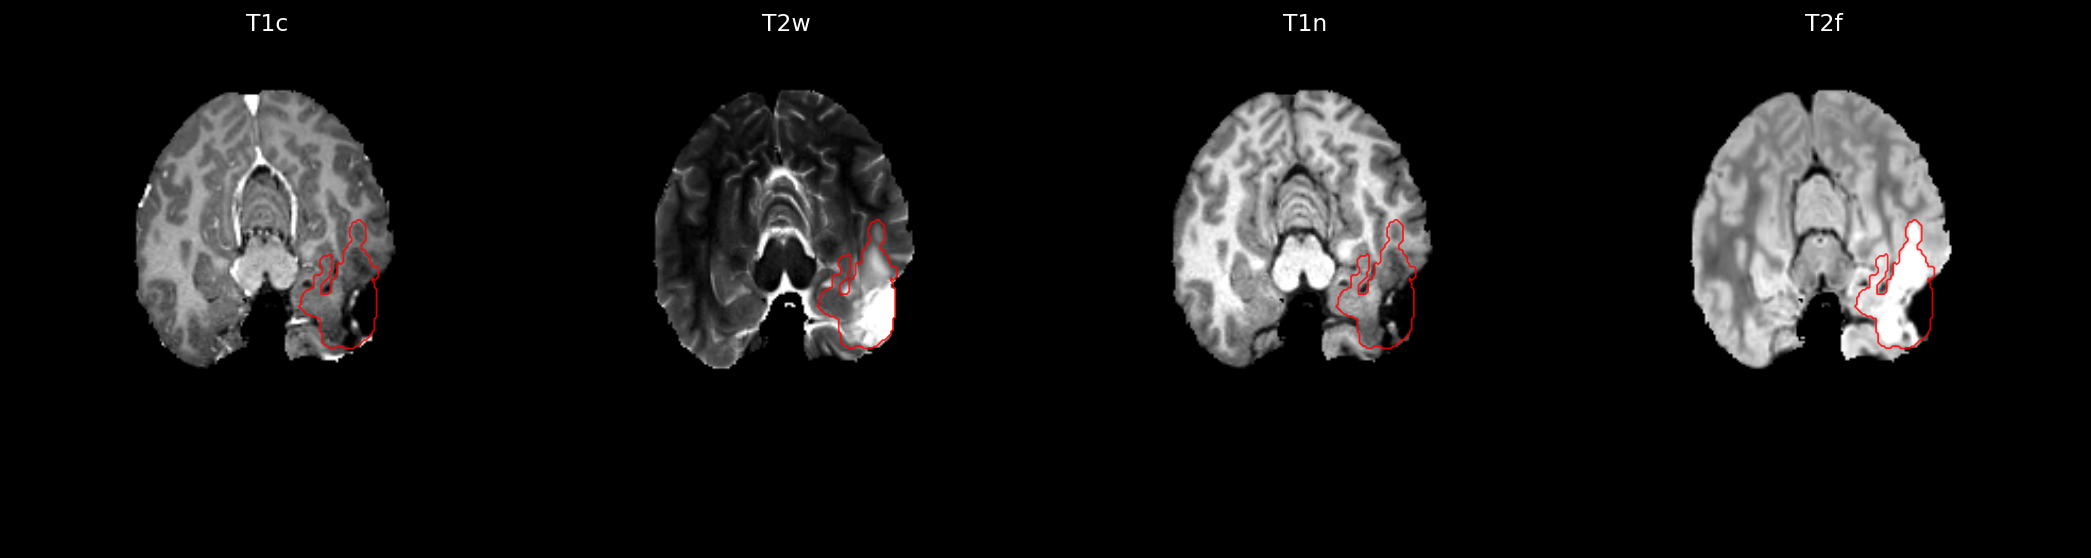
\includegraphics[width=\linewidth]{mri_slices/case_08_mri.png}
\end{center}
{\footnotesize\centering\textit{Red contour = tumor mask. Left to right: T1c, T2w, T1n, T2f (axial slice through tumor center).}\\}

\sectionbar{Proposed Treatment Plans for Next Interval}
{\footnotesize\textit{One option is the actual physician-prescribed regimen; the other is an AI-generated candidate. You do not know which is which.}}

\begin{tcolorbox}[colback=optionA,colframe=optionA!60!black,arc=3pt,title={\textbf{Treatment Option A}},fonttitle=\normalsize\bfseries]
  \begin{itemize}[leftmargin=1.5em,itemsep=1pt,topsep=0pt]
    \item \textbf{RT}: 54.0\,Gy / 30 fractions
    \item \textbf{Chemo}: Temozolomide (continuous)
    \item \textbf{Adjuvant}: Temozolomide $\times$6 cycles (q28d)
  \end{itemize}
\end{tcolorbox}

\begin{tcolorbox}[colback=optionB,colframe=optionB!60!black,arc=3pt,title={\textbf{Treatment Option B}},fonttitle=\normalsize\bfseries]
  \begin{itemize}[leftmargin=1.5em,itemsep=1pt,topsep=0pt]
    \item \textbf{RT}: 60.0\,Gy / 30 fractions
    \item \textbf{Chemo}: Temozolomide (continuous)
  \end{itemize}
\end{tcolorbox}

\sectionbar{Expert Judgment (circle or mark ONE)}
\begin{enumerate}[label=\alph*.,leftmargin=2em,itemsep=4pt,topsep=2pt]
  \item[\checkbox] \textbf{Option A} is more clinically reasonable
  \item[\checkbox] \textbf{Option B} is more clinically reasonable
  \item[\checkbox] Both options are \textbf{clinically equivalent} / acceptable
\end{enumerate}

\sectionbar{Confidence Level \normalfont\small(1 = Very uncertain \quad 5 = Very confident)}
\quad $\checkbox$~1 \qquad $\checkbox$~2 \qquad $\checkbox$~3 \qquad $\checkbox$~4 \qquad $\checkbox$~5

\sectionbar{Optional Comment}
\vspace{1.5cm}\hrule\vspace{0.8cm}\hrule

{\footnotesize\textcolor{gray}{\hfill Generated: 2026-05-08 \quad Study ID: CLARITY-BLIND-08}}
\newpage

\begin{tcolorbox}[colback=headerblue,colframe=headerblue,arc=3pt]
  \color{white}\large\bfseries
  Case 09 \hfill TP1 $\rightarrow$ TP3
\end{tcolorbox}
{\footnotesize\textit{Patient identity anonymized. Do not attempt to de-identify.}}

\sectionbar{Patient Summary}
\begin{tabular}{@{}p{5.5cm}p{10cm}@{}}
  \textbf{\small Age / Sex:} & {\small 43 / Female} \\
  \textbf{\small Race:} & {\small White} \\
  \textbf{\small Diagnosis:} & {\small OLIGODENDRO-GLIOMA, WHO Grade 2} \\
  \textbf{\small Days from diagnosis:} & {\small 104} \\
  \textbf{\small Disease status:} & {\small No prior progression} \\
  \textbf{\small Key molecular markers:} & {\small IDH1 mut;  MGMT methylated;  TERT mut;  1p/19q codeleted} \\
  \textbf{\small Interval to next scan:} & {\small 132 days} \\
\end{tabular}

\sectionbar{Prior Treatment (at pre-scan timepoint)}
\begin{itemize}[leftmargin=1.5em,itemsep=0pt,topsep=2pt]
  \item \textbf{RT}: 54.0\,Gy / 30 fractions
\end{itemize}

\sectionbar{MRI at Pre-treatment Timepoint}
\begin{center}
  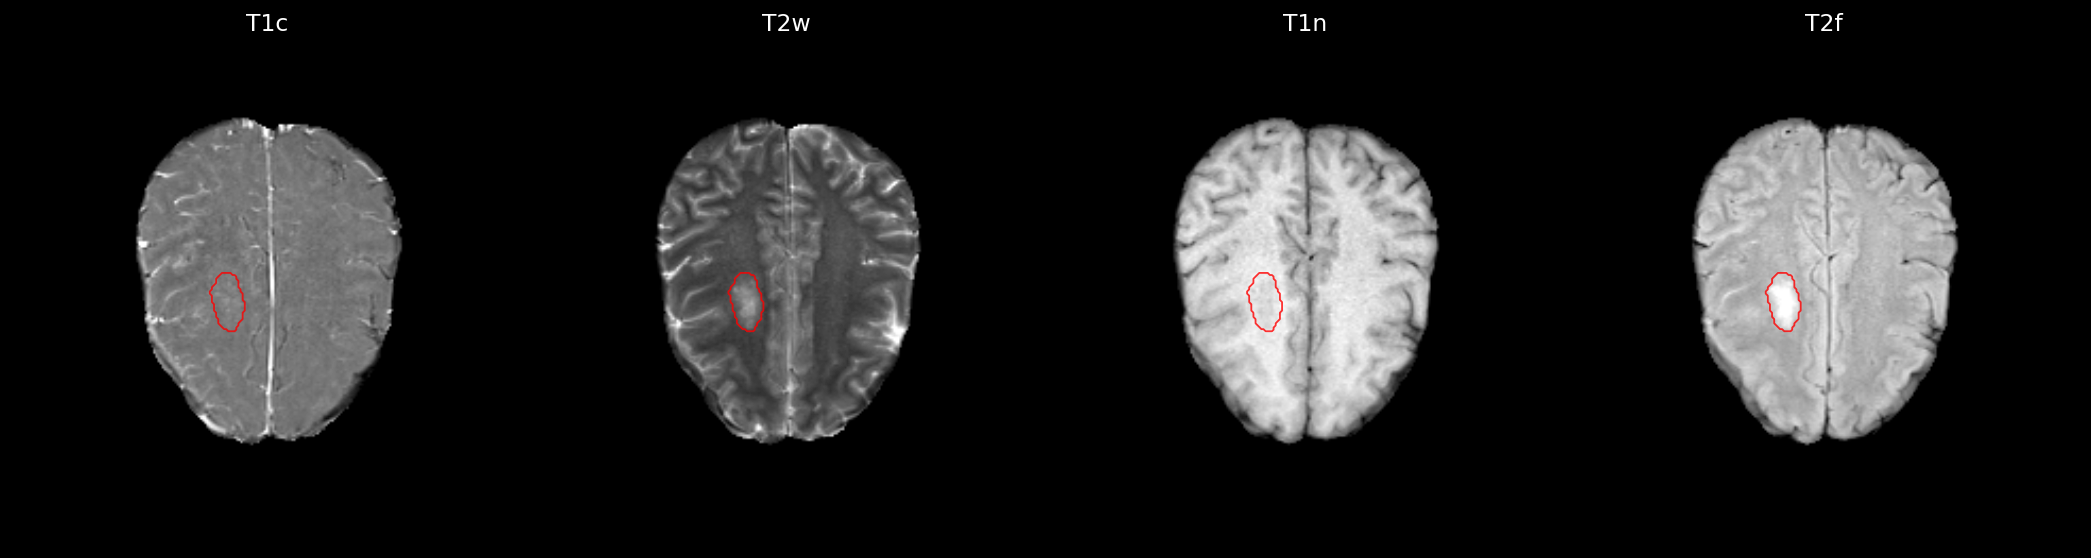
\includegraphics[width=\linewidth]{mri_slices/case_09_mri.png}
\end{center}
{\footnotesize\centering\textit{Red contour = tumor mask. Left to right: T1c, T2w, T1n, T2f (axial slice through tumor center).}\\}

\sectionbar{Proposed Treatment Plans for Next Interval}
{\footnotesize\textit{One option is the actual physician-prescribed regimen; the other is an AI-generated candidate. You do not know which is which.}}

\begin{tcolorbox}[colback=optionA,colframe=optionA!60!black,arc=3pt,title={\textbf{Treatment Option A}},fonttitle=\normalsize\bfseries]
  \begin{itemize}[leftmargin=1.5em,itemsep=1pt,topsep=0pt]
    \item \textbf{Adjuvant}: PCV $\times$6 cycles (q42d)
  \end{itemize}
\end{tcolorbox}

\begin{tcolorbox}[colback=optionB,colframe=optionB!60!black,arc=3pt,title={\textbf{Treatment Option B}},fonttitle=\normalsize\bfseries]
  \begin{itemize}[leftmargin=1.5em,itemsep=1pt,topsep=0pt]
    \item \textbf{RT}: 54.0\,Gy / 30 fractions
    \item \textbf{Adjuvant}: PCV $\times$3 cycles (q42d)
  \end{itemize}
\end{tcolorbox}

\sectionbar{Expert Judgment (circle or mark ONE)}
\begin{enumerate}[label=\alph*.,leftmargin=2em,itemsep=4pt,topsep=2pt]
  \item[\checkbox] \textbf{Option A} is more clinically reasonable
  \item[\checkbox] \textbf{Option B} is more clinically reasonable
  \item[\checkbox] Both options are \textbf{clinically equivalent} / acceptable
\end{enumerate}

\sectionbar{Confidence Level \normalfont\small(1 = Very uncertain \quad 5 = Very confident)}
\quad $\checkbox$~1 \qquad $\checkbox$~2 \qquad $\checkbox$~3 \qquad $\checkbox$~4 \qquad $\checkbox$~5

\sectionbar{Optional Comment}
\vspace{1.5cm}\hrule\vspace{0.8cm}\hrule

{\footnotesize\textcolor{gray}{\hfill Generated: 2026-05-08 \quad Study ID: CLARITY-BLIND-09}}
\newpage

\begin{tcolorbox}[colback=headerblue,colframe=headerblue,arc=3pt]
  \color{white}\large\bfseries
  Case 10 \hfill TP1 $\rightarrow$ TP2
\end{tcolorbox}
{\footnotesize\textit{Patient identity anonymized. Do not attempt to de-identify.}}

\sectionbar{Patient Summary}
\begin{tabular}{@{}p{5.5cm}p{10cm}@{}}
  \textbf{\small Age / Sex:} & {\small 54 / Male} \\
  \textbf{\small Race:} & {\small White} \\
  \textbf{\small Diagnosis:} & {\small GBM, WHO Grade 4} \\
  \textbf{\small Days from diagnosis:} & {\small 44} \\
  \textbf{\small Disease status:} & {\small Progression documented} \\
  \textbf{\small Key molecular markers:} & {\small IDH1 WT;  IDH2 WT;  MGMT unmethylated} \\
  \textbf{\small Interval to next scan:} & {\small 103 days} \\
\end{tabular}

\sectionbar{Prior Treatment (at pre-scan timepoint)}
\begin{itemize}[leftmargin=1.5em,itemsep=0pt,topsep=2pt]
  \item \textbf{RT}: 60.0\,Gy / 30 fractions
  \item \textbf{Chemo}: Temozolomide (continuous)
\end{itemize}

\sectionbar{MRI at Pre-treatment Timepoint}
\begin{center}
  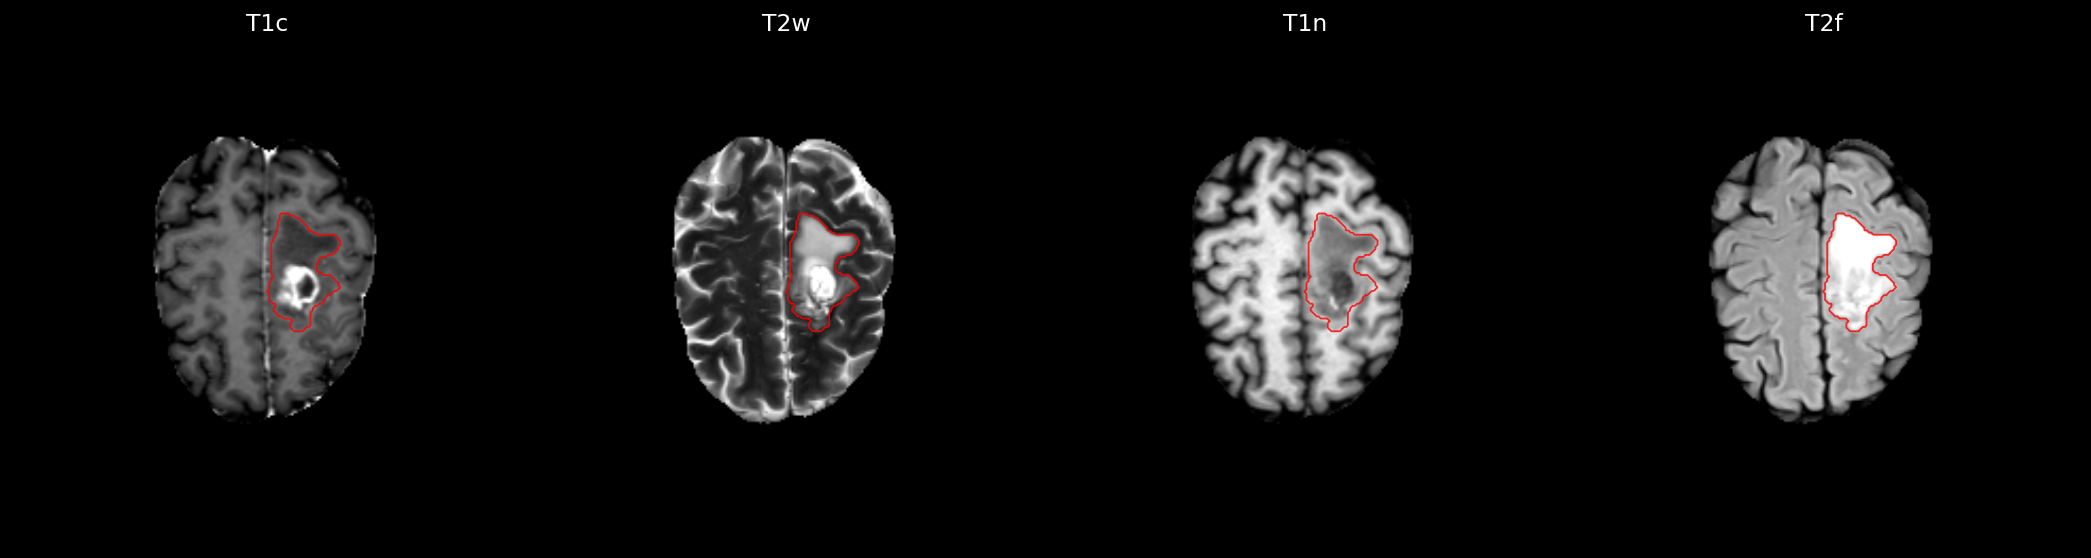
\includegraphics[width=\linewidth]{mri_slices/case_10_mri.png}
\end{center}
{\footnotesize\centering\textit{Red contour = tumor mask. Left to right: T1c, T2w, T1n, T2f (axial slice through tumor center).}\\}

\sectionbar{Proposed Treatment Plans for Next Interval}
{\footnotesize\textit{One option is the actual physician-prescribed regimen; the other is an AI-generated candidate. You do not know which is which.}}

\begin{tcolorbox}[colback=optionA,colframe=optionA!60!black,arc=3pt,title={\textbf{Treatment Option A}},fonttitle=\normalsize\bfseries]
  \begin{itemize}[leftmargin=1.5em,itemsep=1pt,topsep=0pt]
    \item \textbf{Adjuvant}: Temozolomide $\times$6 cycles (q28d)
    \item \textbf{Other}: Optune TTF (continuous)
  \end{itemize}
\end{tcolorbox}

\begin{tcolorbox}[colback=optionB,colframe=optionB!60!black,arc=3pt,title={\textbf{Treatment Option B}},fonttitle=\normalsize\bfseries]
  \begin{itemize}[leftmargin=1.5em,itemsep=1pt,topsep=0pt]
    \item \textbf{Adjuvant}: Temozolomide $\times$4 cycles (q28d)
    \item \textbf{Other}: optune ttf (continuous)
  \end{itemize}
\end{tcolorbox}

\sectionbar{Expert Judgment (circle or mark ONE)}
\begin{enumerate}[label=\alph*.,leftmargin=2em,itemsep=4pt,topsep=2pt]
  \item[\checkbox] \textbf{Option A} is more clinically reasonable
  \item[\checkbox] \textbf{Option B} is more clinically reasonable
  \item[\checkbox] Both options are \textbf{clinically equivalent} / acceptable
\end{enumerate}

\sectionbar{Confidence Level \normalfont\small(1 = Very uncertain \quad 5 = Very confident)}
\quad $\checkbox$~1 \qquad $\checkbox$~2 \qquad $\checkbox$~3 \qquad $\checkbox$~4 \qquad $\checkbox$~5

\sectionbar{Optional Comment}
\vspace{1.5cm}\hrule\vspace{0.8cm}\hrule

{\footnotesize\textcolor{gray}{\hfill Generated: 2026-05-08 \quad Study ID: CLARITY-BLIND-10}}
\newpage

\begin{tcolorbox}[colback=headerblue,colframe=headerblue,arc=3pt]
  \color{white}\large\bfseries
  Case 11 \hfill TP1 $\rightarrow$ TP3
\end{tcolorbox}
{\footnotesize\textit{Patient identity anonymized. Do not attempt to de-identify.}}

\sectionbar{Patient Summary}
\begin{tabular}{@{}p{5.5cm}p{10cm}@{}}
  \textbf{\small Age / Sex:} & {\small 32 / Female} \\
  \textbf{\small Race:} & {\small White} \\
  \textbf{\small Diagnosis:} & {\small ASTROCYTOMA, WHO Grade 2} \\
  \textbf{\small Days from diagnosis:} & {\small 107} \\
  \textbf{\small Disease status:} & {\small Progression documented} \\
  \textbf{\small Key molecular markers:} & {\small IDH1 WT;  IDH2 WT} \\
  \textbf{\small Interval to next scan:} & {\small 183 days} \\
\end{tabular}

\sectionbar{Prior Treatment (at pre-scan timepoint)}
\begin{itemize}[leftmargin=1.5em,itemsep=0pt,topsep=2pt]
  \item \textit{Observation / No active therapy}
\end{itemize}

\sectionbar{MRI at Pre-treatment Timepoint}
\begin{center}
  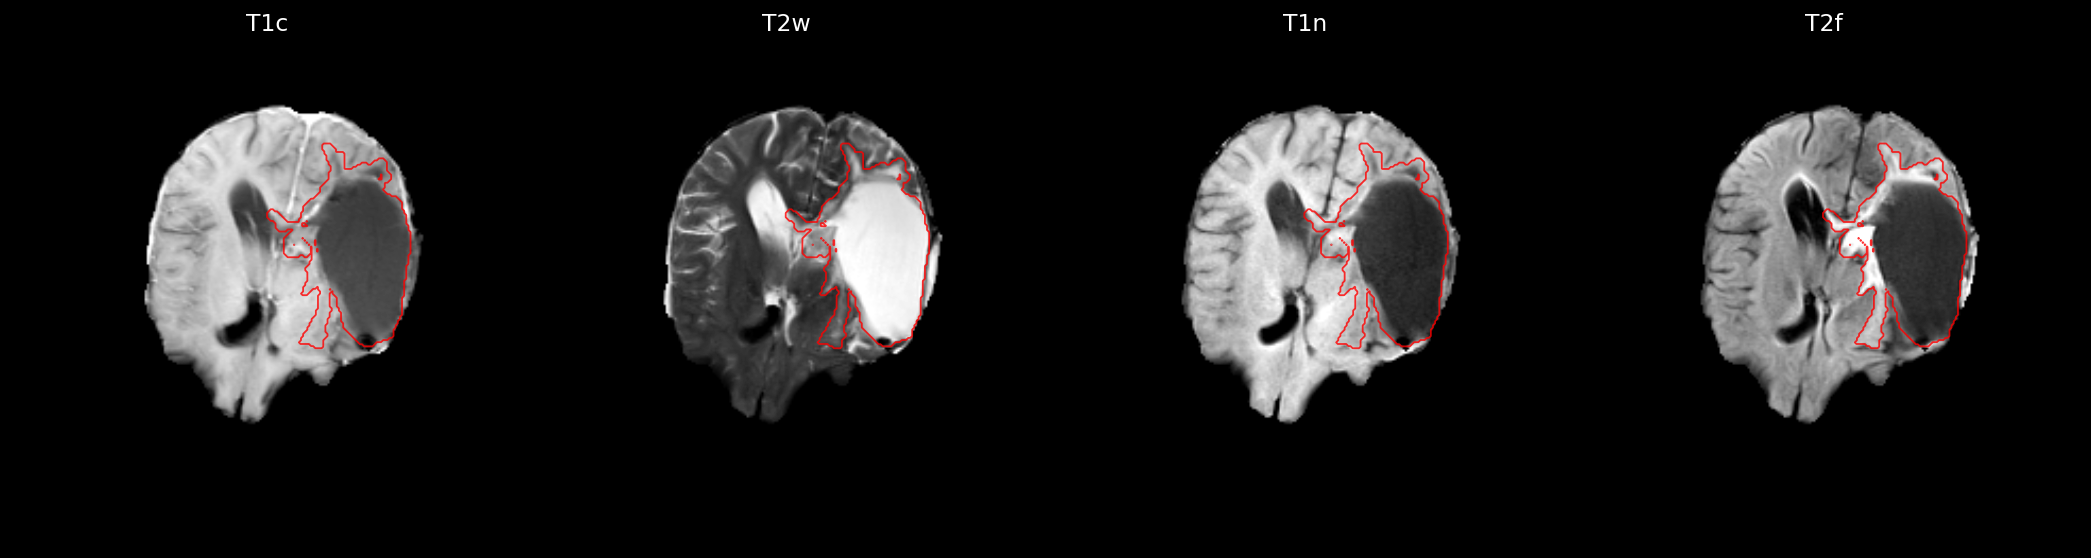
\includegraphics[width=\linewidth]{mri_slices/case_11_mri.png}
\end{center}
{\footnotesize\centering\textit{Red contour = tumor mask. Left to right: T1c, T2w, T1n, T2f (axial slice through tumor center).}\\}

\sectionbar{Proposed Treatment Plans for Next Interval}
{\footnotesize\textit{One option is the actual physician-prescribed regimen; the other is an AI-generated candidate. You do not know which is which.}}

\begin{tcolorbox}[colback=optionA,colframe=optionA!60!black,arc=3pt,title={\textbf{Treatment Option A}},fonttitle=\normalsize\bfseries]
  \begin{itemize}[leftmargin=1.5em,itemsep=1pt,topsep=0pt]
    \item \textbf{Adjuvant}: PCV $\times$6 cycles (q56d)
  \end{itemize}
\end{tcolorbox}

\begin{tcolorbox}[colback=optionB,colframe=optionB!60!black,arc=3pt,title={\textbf{Treatment Option B}},fonttitle=\normalsize\bfseries]
  \begin{itemize}[leftmargin=1.5em,itemsep=1pt,topsep=0pt]
    \item \textbf{RT}: 60.0\,Gy / 30 fractions
    \item \textbf{Chemo}: Temozolomide (continuous)
    \item \textbf{Adjuvant}: Temozolomide $\times$6 cycles (q28d)
  \end{itemize}
\end{tcolorbox}

\sectionbar{Expert Judgment (circle or mark ONE)}
\begin{enumerate}[label=\alph*.,leftmargin=2em,itemsep=4pt,topsep=2pt]
  \item[\checkbox] \textbf{Option A} is more clinically reasonable
  \item[\checkbox] \textbf{Option B} is more clinically reasonable
  \item[\checkbox] Both options are \textbf{clinically equivalent} / acceptable
\end{enumerate}

\sectionbar{Confidence Level \normalfont\small(1 = Very uncertain \quad 5 = Very confident)}
\quad $\checkbox$~1 \qquad $\checkbox$~2 \qquad $\checkbox$~3 \qquad $\checkbox$~4 \qquad $\checkbox$~5

\sectionbar{Optional Comment}
\vspace{1.5cm}\hrule\vspace{0.8cm}\hrule

{\footnotesize\textcolor{gray}{\hfill Generated: 2026-05-08 \quad Study ID: CLARITY-BLIND-11}}
\newpage

\begin{tcolorbox}[colback=headerblue,colframe=headerblue,arc=3pt]
  \color{white}\large\bfseries
  Case 12 \hfill TP1 $\rightarrow$ TP2
\end{tcolorbox}
{\footnotesize\textit{Patient identity anonymized. Do not attempt to de-identify.}}

\sectionbar{Patient Summary}
\begin{tabular}{@{}p{5.5cm}p{10cm}@{}}
  \textbf{\small Age / Sex:} & {\small 53 / Male} \\
  \textbf{\small Race:} & {\small White} \\
  \textbf{\small Diagnosis:} & {\small GBM, WHO Grade 4} \\
  \textbf{\small Days from diagnosis:} & {\small 89} \\
  \textbf{\small Disease status:} & {\small Progression documented} \\
  \textbf{\small Key molecular markers:} & {\small IDH1 WT;  IDH2 WT;  MGMT methylated} \\
  \textbf{\small Interval to next scan:} & {\small 71 days} \\
\end{tabular}

\sectionbar{Prior Treatment (at pre-scan timepoint)}
\begin{itemize}[leftmargin=1.5em,itemsep=0pt,topsep=2pt]
  \item \textbf{RT}: ?\,Gy / ? fractions
  \item \textbf{Chemo}: Temozolomide (continuous)
\end{itemize}

\sectionbar{MRI at Pre-treatment Timepoint}
\begin{center}
  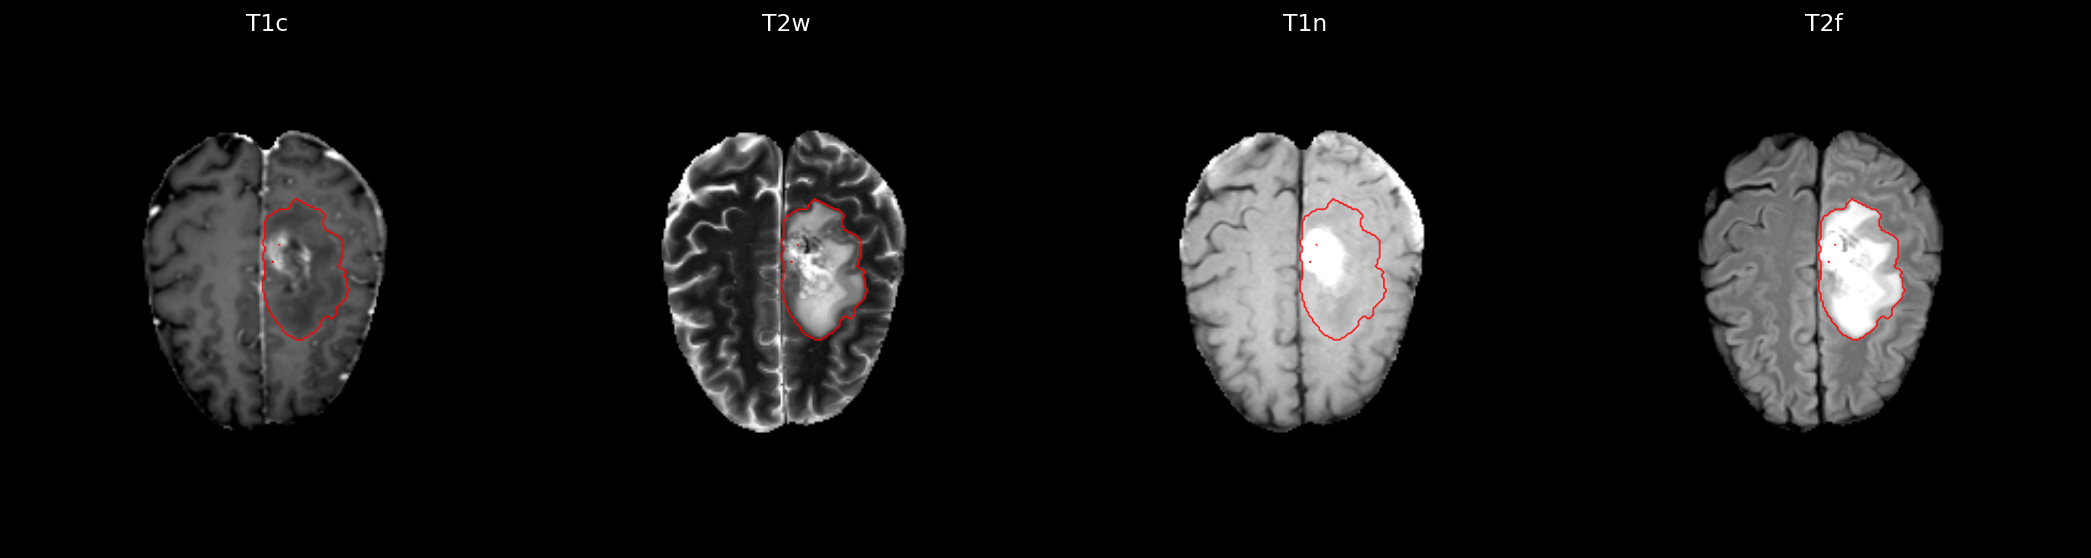
\includegraphics[width=\linewidth]{mri_slices/case_12_mri.png}
\end{center}
{\footnotesize\centering\textit{Red contour = tumor mask. Left to right: T1c, T2w, T1n, T2f (axial slice through tumor center).}\\}

\sectionbar{Proposed Treatment Plans for Next Interval}
{\footnotesize\textit{One option is the actual physician-prescribed regimen; the other is an AI-generated candidate. You do not know which is which.}}

\begin{tcolorbox}[colback=optionA,colframe=optionA!60!black,arc=3pt,title={\textbf{Treatment Option A}},fonttitle=\normalsize\bfseries]
  \begin{itemize}[leftmargin=1.5em,itemsep=1pt,topsep=0pt]
    \item \textbf{Adjuvant}: Temozolomide $\times$7 cycles (q28d)
  \end{itemize}
\end{tcolorbox}

\begin{tcolorbox}[colback=optionB,colframe=optionB!60!black,arc=3pt,title={\textbf{Treatment Option B}},fonttitle=\normalsize\bfseries]
  \begin{itemize}[leftmargin=1.5em,itemsep=1pt,topsep=0pt]
    \item \textbf{Adjuvant}: Temozolomide $\times$6 cycles (q28d)
    \item \textbf{Other}: Optune TTF (continuous)
  \end{itemize}
\end{tcolorbox}

\sectionbar{Expert Judgment (circle or mark ONE)}
\begin{enumerate}[label=\alph*.,leftmargin=2em,itemsep=4pt,topsep=2pt]
  \item[\checkbox] \textbf{Option A} is more clinically reasonable
  \item[\checkbox] \textbf{Option B} is more clinically reasonable
  \item[\checkbox] Both options are \textbf{clinically equivalent} / acceptable
\end{enumerate}

\sectionbar{Confidence Level \normalfont\small(1 = Very uncertain \quad 5 = Very confident)}
\quad $\checkbox$~1 \qquad $\checkbox$~2 \qquad $\checkbox$~3 \qquad $\checkbox$~4 \qquad $\checkbox$~5

\sectionbar{Optional Comment}
\vspace{1.5cm}\hrule\vspace{0.8cm}\hrule

{\footnotesize\textcolor{gray}{\hfill Generated: 2026-05-08 \quad Study ID: CLARITY-BLIND-12}}
\newpage

\begin{tcolorbox}[colback=headerblue,colframe=headerblue,arc=3pt]
  \color{white}\large\bfseries
  Case 13 \hfill TP1 $\rightarrow$ TP3
\end{tcolorbox}
{\footnotesize\textit{Patient identity anonymized. Do not attempt to de-identify.}}

\sectionbar{Patient Summary}
\begin{tabular}{@{}p{5.5cm}p{10cm}@{}}
  \textbf{\small Age / Sex:} & {\small 56 / Female} \\
  \textbf{\small Race:} & {\small White} \\
  \textbf{\small Diagnosis:} & {\small GBM, WHO Grade 4} \\
  \textbf{\small Days from diagnosis:} & {\small 89} \\
  \textbf{\small Disease status:} & {\small No prior progression} \\
  \textbf{\small Key molecular markers:} & {\small MGMT unmethylated;  CDKN2A/B del} \\
  \textbf{\small Interval to next scan:} & {\small 119 days} \\
\end{tabular}

\sectionbar{Prior Treatment (at pre-scan timepoint)}
\begin{itemize}[leftmargin=1.5em,itemsep=0pt,topsep=2pt]
  \item \textbf{RT}: 60.0\,Gy / 30 fractions
  \item \textbf{Chemo}: Temozolomide (continuous)
\end{itemize}

\sectionbar{MRI at Pre-treatment Timepoint}
\begin{center}
  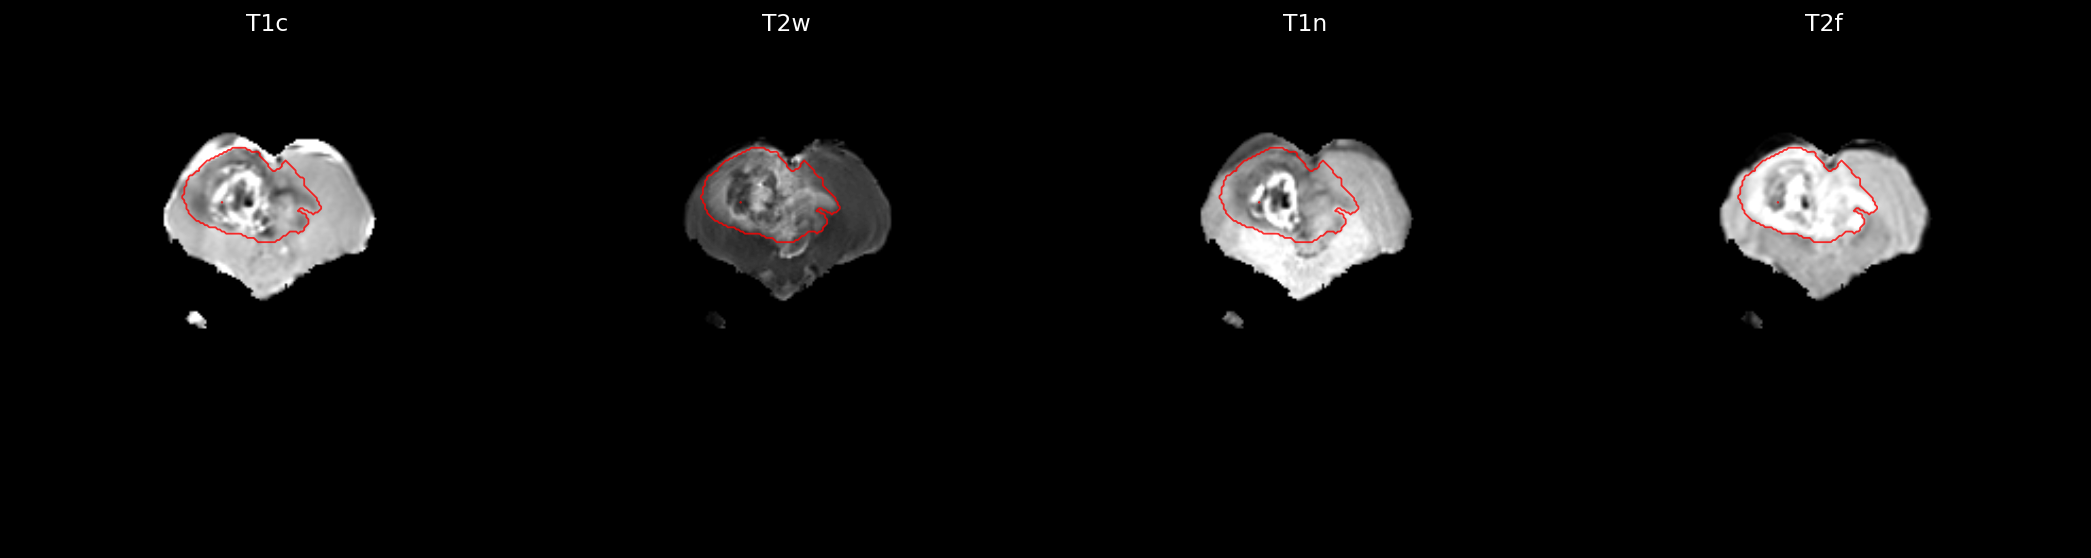
\includegraphics[width=\linewidth]{mri_slices/case_13_mri.png}
\end{center}
{\footnotesize\centering\textit{Red contour = tumor mask. Left to right: T1c, T2w, T1n, T2f (axial slice through tumor center).}\\}

\sectionbar{Proposed Treatment Plans for Next Interval}
{\footnotesize\textit{One option is the actual physician-prescribed regimen; the other is an AI-generated candidate. You do not know which is which.}}

\begin{tcolorbox}[colback=optionA,colframe=optionA!60!black,arc=3pt,title={\textbf{Treatment Option A}},fonttitle=\normalsize\bfseries]
  \begin{itemize}[leftmargin=1.5em,itemsep=1pt,topsep=0pt]
    \item \textbf{Adjuvant}: Temozolomide $\times$6 cycles (q28d)
    \item \textbf{Other}: Optune TTF (continuous)
  \end{itemize}
\end{tcolorbox}

\begin{tcolorbox}[colback=optionB,colframe=optionB!60!black,arc=3pt,title={\textbf{Treatment Option B}},fonttitle=\normalsize\bfseries]
  \begin{itemize}[leftmargin=1.5em,itemsep=1pt,topsep=0pt]
    \item \textbf{Adjuvant}: Temozolomide $\times$10 cycles (q28d)
    \item \textbf{Other}: optune ttf (continuous)
  \end{itemize}
\end{tcolorbox}

\sectionbar{Expert Judgment (circle or mark ONE)}
\begin{enumerate}[label=\alph*.,leftmargin=2em,itemsep=4pt,topsep=2pt]
  \item[\checkbox] \textbf{Option A} is more clinically reasonable
  \item[\checkbox] \textbf{Option B} is more clinically reasonable
  \item[\checkbox] Both options are \textbf{clinically equivalent} / acceptable
\end{enumerate}

\sectionbar{Confidence Level \normalfont\small(1 = Very uncertain \quad 5 = Very confident)}
\quad $\checkbox$~1 \qquad $\checkbox$~2 \qquad $\checkbox$~3 \qquad $\checkbox$~4 \qquad $\checkbox$~5

\sectionbar{Optional Comment}
\vspace{1.5cm}\hrule\vspace{0.8cm}\hrule

{\footnotesize\textcolor{gray}{\hfill Generated: 2026-05-08 \quad Study ID: CLARITY-BLIND-13}}
\newpage

\begin{tcolorbox}[colback=headerblue,colframe=headerblue,arc=3pt]
  \color{white}\large\bfseries
  Case 14 \hfill TP1 $\rightarrow$ TP2
\end{tcolorbox}
{\footnotesize\textit{Patient identity anonymized. Do not attempt to de-identify.}}

\sectionbar{Patient Summary}
\begin{tabular}{@{}p{5.5cm}p{10cm}@{}}
  \textbf{\small Age / Sex:} & {\small 37 / Male} \\
  \textbf{\small Race:} & {\small White} \\
  \textbf{\small Diagnosis:} & {\small GBM, WHO Grade 4} \\
  \textbf{\small Days from diagnosis:} & {\small 68} \\
  \textbf{\small Disease status:} & {\small Progression documented} \\
  \textbf{\small Key molecular markers:} & {\small IDH1 WT;  IDH2 WT;  MGMT unmethylated} \\
  \textbf{\small Interval to next scan:} & {\small 73 days} \\
\end{tabular}

\sectionbar{Prior Treatment (at pre-scan timepoint)}
\begin{itemize}[leftmargin=1.5em,itemsep=0pt,topsep=2pt]
  \item \textbf{RT}: 40.0\,Gy / 15 fractions
  \item \textbf{Chemo}: Temozolomide (continuous)
  \item \textbf{Adjuvant}: Temozolomide $\times$2 cycles (q28d)
\end{itemize}

\sectionbar{MRI at Pre-treatment Timepoint}
\begin{center}
  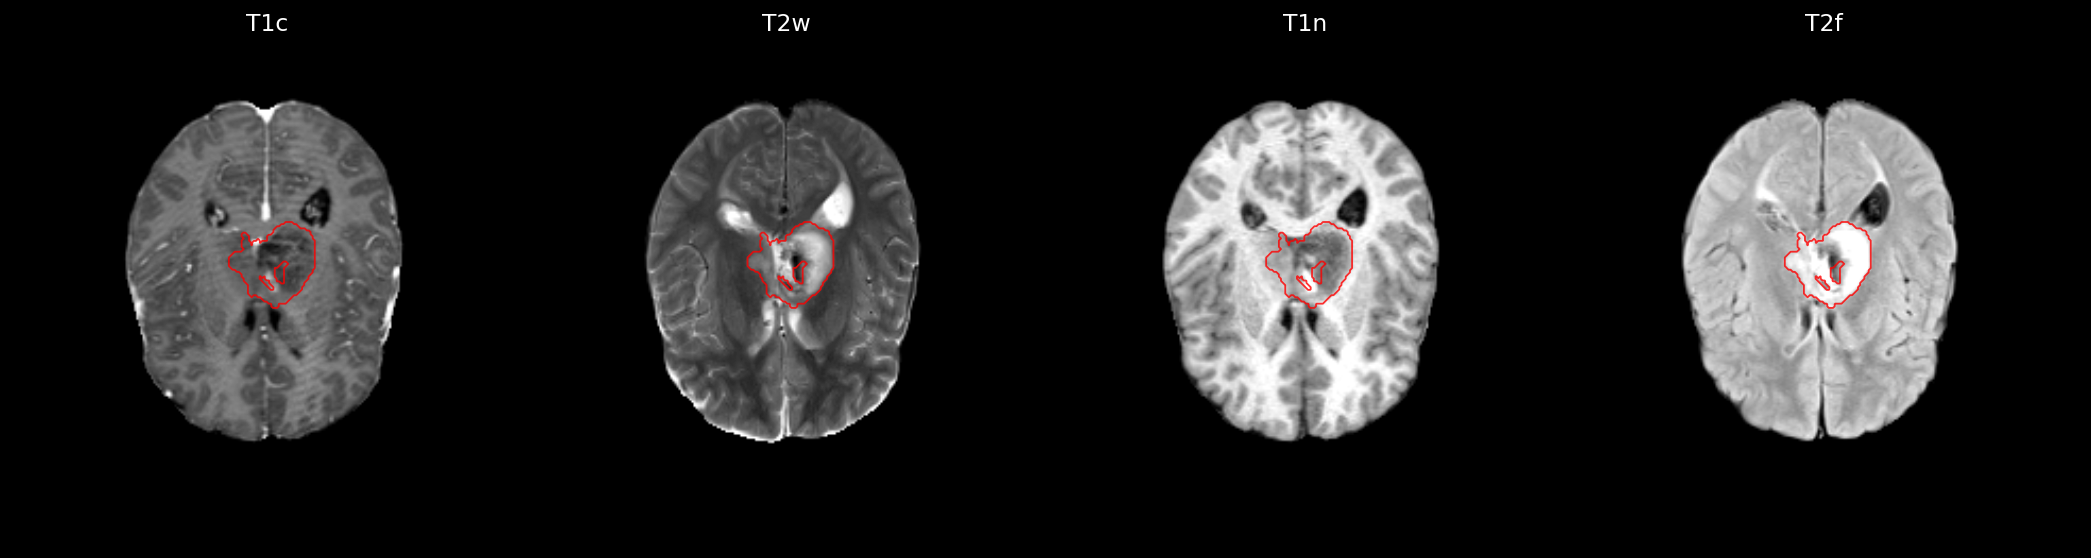
\includegraphics[width=\linewidth]{mri_slices/case_14_mri.png}
\end{center}
{\footnotesize\centering\textit{Red contour = tumor mask. Left to right: T1c, T2w, T1n, T2f (axial slice through tumor center).}\\}

\sectionbar{Proposed Treatment Plans for Next Interval}
{\footnotesize\textit{One option is the actual physician-prescribed regimen; the other is an AI-generated candidate. You do not know which is which.}}

\begin{tcolorbox}[colback=optionA,colframe=optionA!60!black,arc=3pt,title={\textbf{Treatment Option A}},fonttitle=\normalsize\bfseries]
  \begin{itemize}[leftmargin=1.5em,itemsep=1pt,topsep=0pt]
    \item \textbf{Adjuvant}: Temozolomide $\times$4 cycles (q28d)
    \item \textbf{Other}: Optune TTF (continuous)
  \end{itemize}
\end{tcolorbox}

\begin{tcolorbox}[colback=optionB,colframe=optionB!60!black,arc=3pt,title={\textbf{Treatment Option B}},fonttitle=\normalsize\bfseries]
  \begin{itemize}[leftmargin=1.5em,itemsep=1pt,topsep=0pt]
    \item \textbf{Immuno}: Avastin $\times$7 cycles (q14d)
    \item \textbf{Adjuvant}: Temozolomide $\times$2 cycles (q28d)
  \end{itemize}
\end{tcolorbox}

\sectionbar{Expert Judgment (circle or mark ONE)}
\begin{enumerate}[label=\alph*.,leftmargin=2em,itemsep=4pt,topsep=2pt]
  \item[\checkbox] \textbf{Option A} is more clinically reasonable
  \item[\checkbox] \textbf{Option B} is more clinically reasonable
  \item[\checkbox] Both options are \textbf{clinically equivalent} / acceptable
\end{enumerate}

\sectionbar{Confidence Level \normalfont\small(1 = Very uncertain \quad 5 = Very confident)}
\quad $\checkbox$~1 \qquad $\checkbox$~2 \qquad $\checkbox$~3 \qquad $\checkbox$~4 \qquad $\checkbox$~5

\sectionbar{Optional Comment}
\vspace{1.5cm}\hrule\vspace{0.8cm}\hrule

{\footnotesize\textcolor{gray}{\hfill Generated: 2026-05-08 \quad Study ID: CLARITY-BLIND-14}}
\newpage

\begin{tcolorbox}[colback=headerblue,colframe=headerblue,arc=3pt]
  \color{white}\large\bfseries
  Case 15 \hfill TP1 $\rightarrow$ TP2
\end{tcolorbox}
{\footnotesize\textit{Patient identity anonymized. Do not attempt to de-identify.}}

\sectionbar{Patient Summary}
\begin{tabular}{@{}p{5.5cm}p{10cm}@{}}
  \textbf{\small Age / Sex:} & {\small 24 / Female} \\
  \textbf{\small Race:} & {\small White} \\
  \textbf{\small Diagnosis:} & {\small DIFFUSE GLIOMA, WHO Grade 4} \\
  \textbf{\small Days from diagnosis:} & {\small 3} \\
  \textbf{\small Disease status:} & {\small Progression documented} \\
  \textbf{\small Key molecular markers:} & {\small IDH1 mut;  MGMT methylated;  TP53 alt} \\
  \textbf{\small Interval to next scan:} & {\small 77 days} \\
\end{tabular}

\sectionbar{Prior Treatment (at pre-scan timepoint)}
\begin{itemize}[leftmargin=1.5em,itemsep=0pt,topsep=2pt]
  \item \textit{Observation / No active therapy}
\end{itemize}

\sectionbar{MRI at Pre-treatment Timepoint}
\begin{center}
  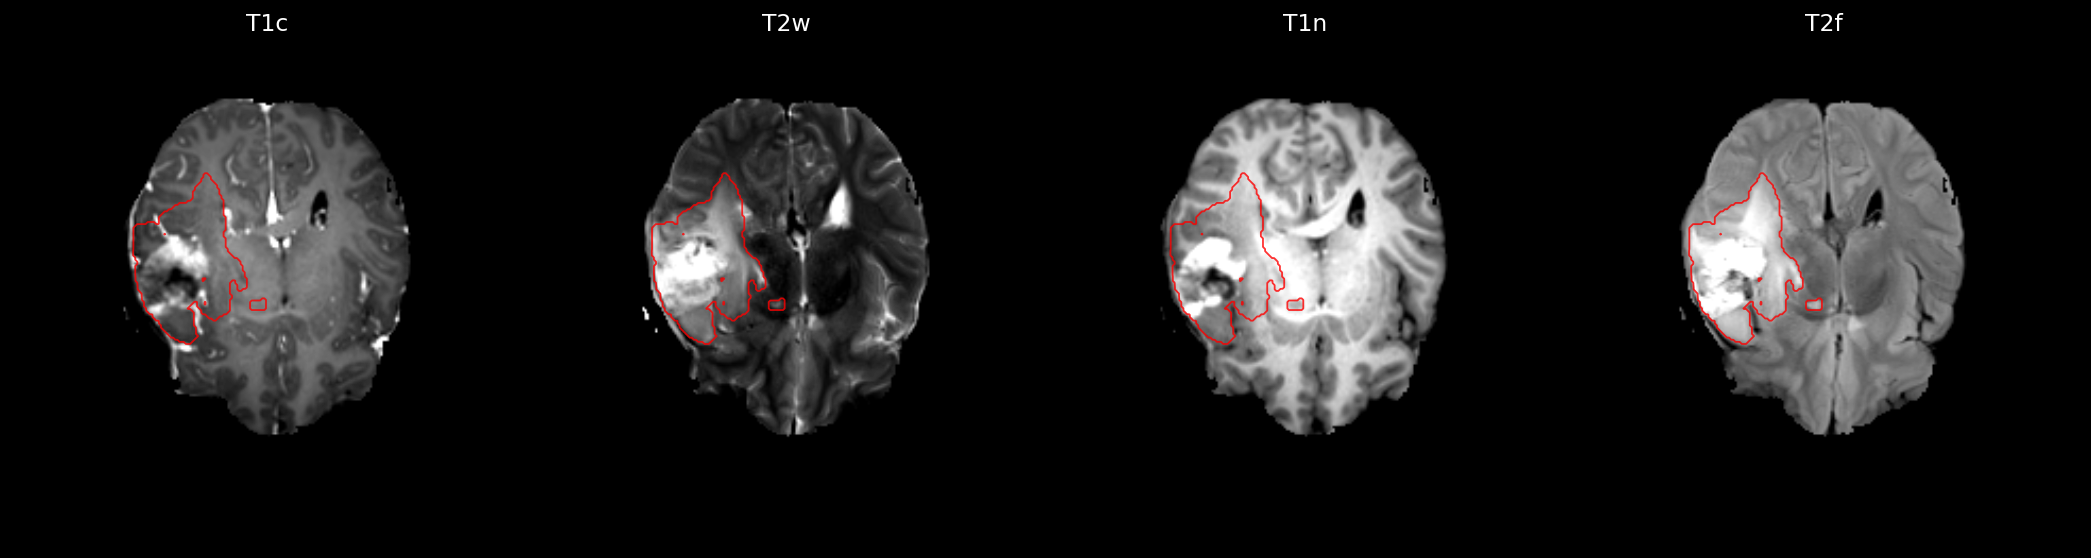
\includegraphics[width=\linewidth]{mri_slices/case_15_mri.png}
\end{center}
{\footnotesize\centering\textit{Red contour = tumor mask. Left to right: T1c, T2w, T1n, T2f (axial slice through tumor center).}\\}

\sectionbar{Proposed Treatment Plans for Next Interval}
{\footnotesize\textit{One option is the actual physician-prescribed regimen; the other is an AI-generated candidate. You do not know which is which.}}

\begin{tcolorbox}[colback=optionA,colframe=optionA!60!black,arc=3pt,title={\textbf{Treatment Option A}},fonttitle=\normalsize\bfseries]
  \begin{itemize}[leftmargin=1.5em,itemsep=1pt,topsep=0pt]
    \item \textbf{RT}: 60.0\,Gy / 30 fractions
    \item \textbf{Chemo}: Temozolomide (continuous)
    \item \textbf{Adjuvant}: Temozolomide $\times$12 cycles (q28d)
    \item \textbf{Other}: Optune TTF (continuous)
  \end{itemize}
\end{tcolorbox}

\begin{tcolorbox}[colback=optionB,colframe=optionB!60!black,arc=3pt,title={\textbf{Treatment Option B}},fonttitle=\normalsize\bfseries]
  \begin{itemize}[leftmargin=1.5em,itemsep=1pt,topsep=0pt]
    \item \textbf{RT}: 60.0\,Gy / 30 fractions
    \item \textbf{Chemo}: Temozolomide (continuous)
    \item \textbf{Adjuvant}: Temozolomide $\times$7 cycles (q28d)
    \item \textbf{Other}: optune ttf (continuous)
  \end{itemize}
\end{tcolorbox}

\sectionbar{Expert Judgment (circle or mark ONE)}
\begin{enumerate}[label=\alph*.,leftmargin=2em,itemsep=4pt,topsep=2pt]
  \item[\checkbox] \textbf{Option A} is more clinically reasonable
  \item[\checkbox] \textbf{Option B} is more clinically reasonable
  \item[\checkbox] Both options are \textbf{clinically equivalent} / acceptable
\end{enumerate}

\sectionbar{Confidence Level \normalfont\small(1 = Very uncertain \quad 5 = Very confident)}
\quad $\checkbox$~1 \qquad $\checkbox$~2 \qquad $\checkbox$~3 \qquad $\checkbox$~4 \qquad $\checkbox$~5

\sectionbar{Optional Comment}
\vspace{1.5cm}\hrule\vspace{0.8cm}\hrule

{\footnotesize\textcolor{gray}{\hfill Generated: 2026-05-08 \quad Study ID: CLARITY-BLIND-15}}
\newpage

\begin{tcolorbox}[colback=headerblue,colframe=headerblue,arc=3pt]
  \color{white}\large\bfseries
  Case 16 \hfill TP1 $\rightarrow$ TP2
\end{tcolorbox}
{\footnotesize\textit{Patient identity anonymized. Do not attempt to de-identify.}}

\sectionbar{Patient Summary}
\begin{tabular}{@{}p{5.5cm}p{10cm}@{}}
  \textbf{\small Age / Sex:} & {\small 59 / Female} \\
  \textbf{\small Race:} & {\small White} \\
  \textbf{\small Diagnosis:} & {\small GBM, WHO Grade 4} \\
  \textbf{\small Days from diagnosis:} & {\small 104} \\
  \textbf{\small Disease status:} & {\small Progression documented} \\
  \textbf{\small Key molecular markers:} & {\small IDH1 WT;  IDH2 WT;  MGMT methylated} \\
  \textbf{\small Interval to next scan:} & {\small 70 days} \\
\end{tabular}

\sectionbar{Prior Treatment (at pre-scan timepoint)}
\begin{itemize}[leftmargin=1.5em,itemsep=0pt,topsep=2pt]
  \item \textbf{RT}: 60.0\,Gy / 30 fractions
  \item \textbf{Chemo}: Temozolomide (continuous)
\end{itemize}

\sectionbar{MRI at Pre-treatment Timepoint}
\begin{center}
  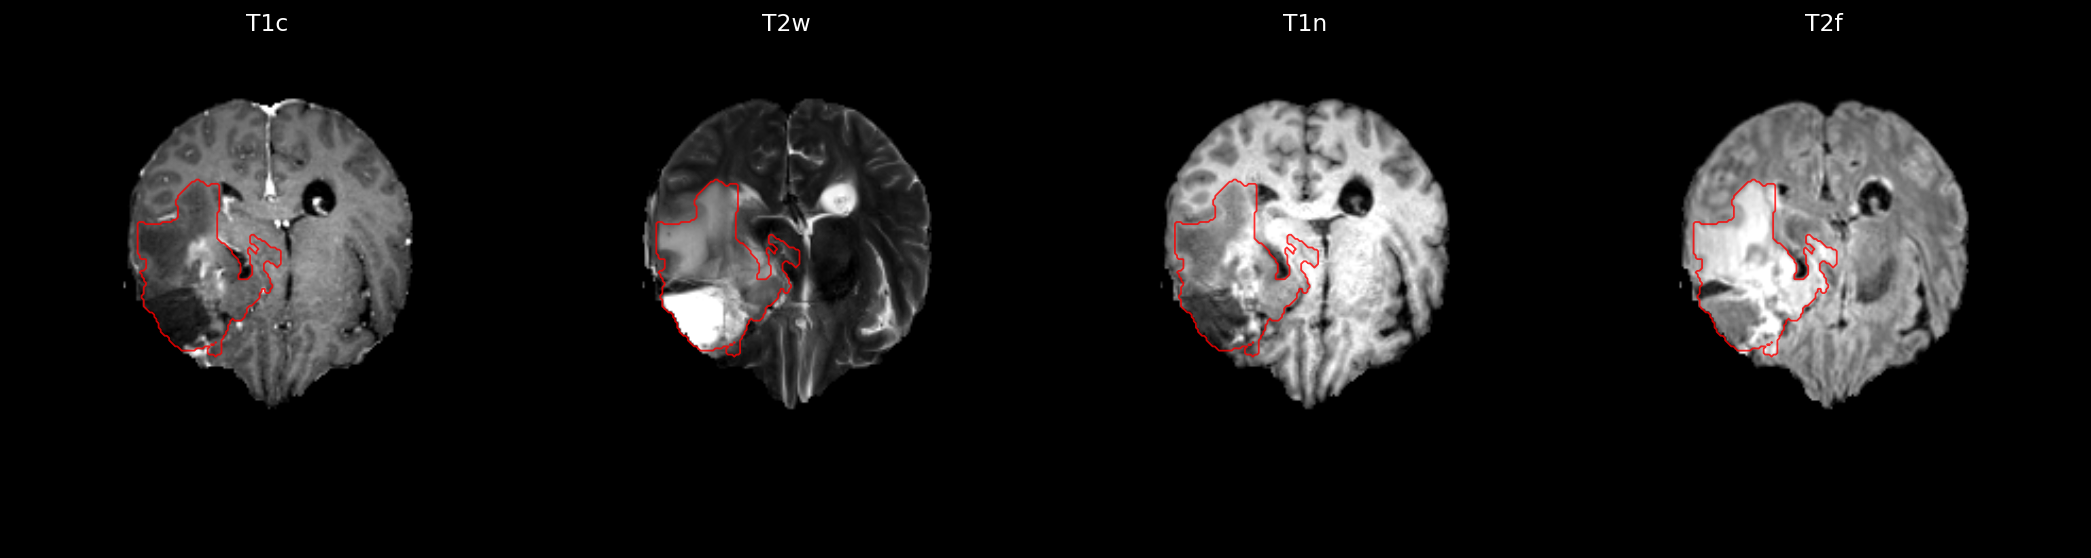
\includegraphics[width=\linewidth]{mri_slices/case_16_mri.png}
\end{center}
{\footnotesize\centering\textit{Red contour = tumor mask. Left to right: T1c, T2w, T1n, T2f (axial slice through tumor center).}\\}

\sectionbar{Proposed Treatment Plans for Next Interval}
{\footnotesize\textit{One option is the actual physician-prescribed regimen; the other is an AI-generated candidate. You do not know which is which.}}

\begin{tcolorbox}[colback=optionA,colframe=optionA!60!black,arc=3pt,title={\textbf{Treatment Option A}},fonttitle=\normalsize\bfseries]
  \begin{itemize}[leftmargin=1.5em,itemsep=1pt,topsep=0pt]
    \item \textbf{Brachy}: 
  \end{itemize}
\end{tcolorbox}

\begin{tcolorbox}[colback=optionB,colframe=optionB!60!black,arc=3pt,title={\textbf{Treatment Option B}},fonttitle=\normalsize\bfseries]
  \begin{itemize}[leftmargin=1.5em,itemsep=1pt,topsep=0pt]
    \item \textbf{Immuno}: Bevacizumab $\times$ongoing cycles (q14d)
    \item \textbf{Adjuvant}: Lomustine (CCNU) $\times$ongoing cycles (q42d)
  \end{itemize}
\end{tcolorbox}

\sectionbar{Expert Judgment (circle or mark ONE)}
\begin{enumerate}[label=\alph*.,leftmargin=2em,itemsep=4pt,topsep=2pt]
  \item[\checkbox] \textbf{Option A} is more clinically reasonable
  \item[\checkbox] \textbf{Option B} is more clinically reasonable
  \item[\checkbox] Both options are \textbf{clinically equivalent} / acceptable
\end{enumerate}

\sectionbar{Confidence Level \normalfont\small(1 = Very uncertain \quad 5 = Very confident)}
\quad $\checkbox$~1 \qquad $\checkbox$~2 \qquad $\checkbox$~3 \qquad $\checkbox$~4 \qquad $\checkbox$~5

\sectionbar{Optional Comment}
\vspace{1.5cm}\hrule\vspace{0.8cm}\hrule

{\footnotesize\textcolor{gray}{\hfill Generated: 2026-05-08 \quad Study ID: CLARITY-BLIND-16}}
\newpage

\begin{tcolorbox}[colback=headerblue,colframe=headerblue,arc=3pt]
  \color{white}\large\bfseries
  Case 17 \hfill TP1 $\rightarrow$ TP2
\end{tcolorbox}
{\footnotesize\textit{Patient identity anonymized. Do not attempt to de-identify.}}

\sectionbar{Patient Summary}
\begin{tabular}{@{}p{5.5cm}p{10cm}@{}}
  \textbf{\small Age / Sex:} & {\small 65 / Female} \\
  \textbf{\small Race:} & {\small White} \\
  \textbf{\small Diagnosis:} & {\small GBM, WHO Grade 4} \\
  \textbf{\small Days from diagnosis:} & {\small 98} \\
  \textbf{\small Disease status:} & {\small Progression documented} \\
  \textbf{\small Key molecular markers:} & {\small IDH1 WT;  IDH2 WT;  MGMT methylated} \\
  \textbf{\small Interval to next scan:} & {\small 77 days} \\
\end{tabular}

\sectionbar{Prior Treatment (at pre-scan timepoint)}
\begin{itemize}[leftmargin=1.5em,itemsep=0pt,topsep=2pt]
  \item \textbf{RT}: 60.0\,Gy / 30 fractions
  \item \textbf{Chemo}: Temozolomide (continuous)
  \item \textbf{Other}: optune ttf (continuous)
\end{itemize}

\sectionbar{MRI at Pre-treatment Timepoint}
\begin{center}
  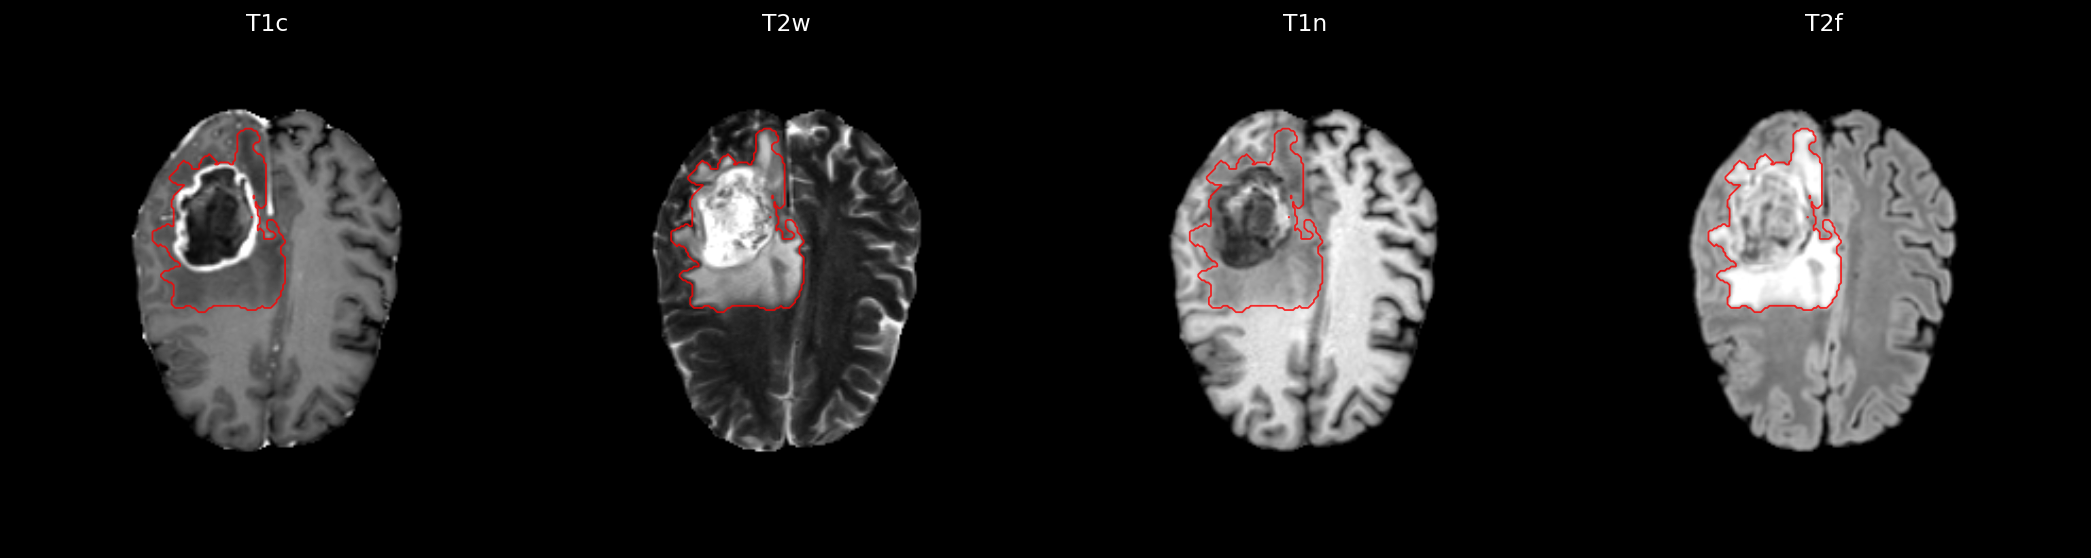
\includegraphics[width=\linewidth]{mri_slices/case_17_mri.png}
\end{center}
{\footnotesize\centering\textit{Red contour = tumor mask. Left to right: T1c, T2w, T1n, T2f (axial slice through tumor center).}\\}

\sectionbar{Proposed Treatment Plans for Next Interval}
{\footnotesize\textit{One option is the actual physician-prescribed regimen; the other is an AI-generated candidate. You do not know which is which.}}

\begin{tcolorbox}[colback=optionA,colframe=optionA!60!black,arc=3pt,title={\textbf{Treatment Option A}},fonttitle=\normalsize\bfseries]
  \begin{itemize}[leftmargin=1.5em,itemsep=1pt,topsep=0pt]
    \item \textbf{Adjuvant}: Temozolomide $\times$2 cycles (q28d)
    \item \textbf{Other}: optune ttf (continuous)
  \end{itemize}
\end{tcolorbox}

\begin{tcolorbox}[colback=optionB,colframe=optionB!60!black,arc=3pt,title={\textbf{Treatment Option B}},fonttitle=\normalsize\bfseries]
  \begin{itemize}[leftmargin=1.5em,itemsep=1pt,topsep=0pt]
    \item \textbf{Immuno}: Bevacizumab $\times$ongoing cycles (q14d)
    \item \textbf{Adjuvant}: Lomustine $\times$ongoing cycles (q42d)
  \end{itemize}
\end{tcolorbox}

\sectionbar{Expert Judgment (circle or mark ONE)}
\begin{enumerate}[label=\alph*.,leftmargin=2em,itemsep=4pt,topsep=2pt]
  \item[\checkbox] \textbf{Option A} is more clinically reasonable
  \item[\checkbox] \textbf{Option B} is more clinically reasonable
  \item[\checkbox] Both options are \textbf{clinically equivalent} / acceptable
\end{enumerate}

\sectionbar{Confidence Level \normalfont\small(1 = Very uncertain \quad 5 = Very confident)}
\quad $\checkbox$~1 \qquad $\checkbox$~2 \qquad $\checkbox$~3 \qquad $\checkbox$~4 \qquad $\checkbox$~5

\sectionbar{Optional Comment}
\vspace{1.5cm}\hrule\vspace{0.8cm}\hrule

{\footnotesize\textcolor{gray}{\hfill Generated: 2026-05-08 \quad Study ID: CLARITY-BLIND-17}}
\newpage

\begin{tcolorbox}[colback=headerblue,colframe=headerblue,arc=3pt]
  \color{white}\large\bfseries
  Case 18 \hfill TP1 $\rightarrow$ TP2
\end{tcolorbox}
{\footnotesize\textit{Patient identity anonymized. Do not attempt to de-identify.}}

\sectionbar{Patient Summary}
\begin{tabular}{@{}p{5.5cm}p{10cm}@{}}
  \textbf{\small Age / Sex:} & {\small 66 / Male} \\
  \textbf{\small Race:} & {\small White} \\
  \textbf{\small Diagnosis:} & {\small GBM, WHO Grade 4} \\
  \textbf{\small Days from diagnosis:} & {\small 90} \\
  \textbf{\small Disease status:} & {\small Progression documented} \\
  \textbf{\small Key molecular markers:} & {\small IDH1 WT;  IDH2 WT;  MGMT methylated;  EGFR amp;  TERT mut} \\
  \textbf{\small Interval to next scan:} & {\small 62 days} \\
\end{tabular}

\sectionbar{Prior Treatment (at pre-scan timepoint)}
\begin{itemize}[leftmargin=1.5em,itemsep=0pt,topsep=2pt]
  \item \textbf{RT}: 60.0\,Gy / 30 fractions
  \item \textbf{Chemo}: Temozolomide (continuous)
  \item \textbf{Other}: optune ttf (continuous)
\end{itemize}

\sectionbar{MRI at Pre-treatment Timepoint}
\begin{center}
  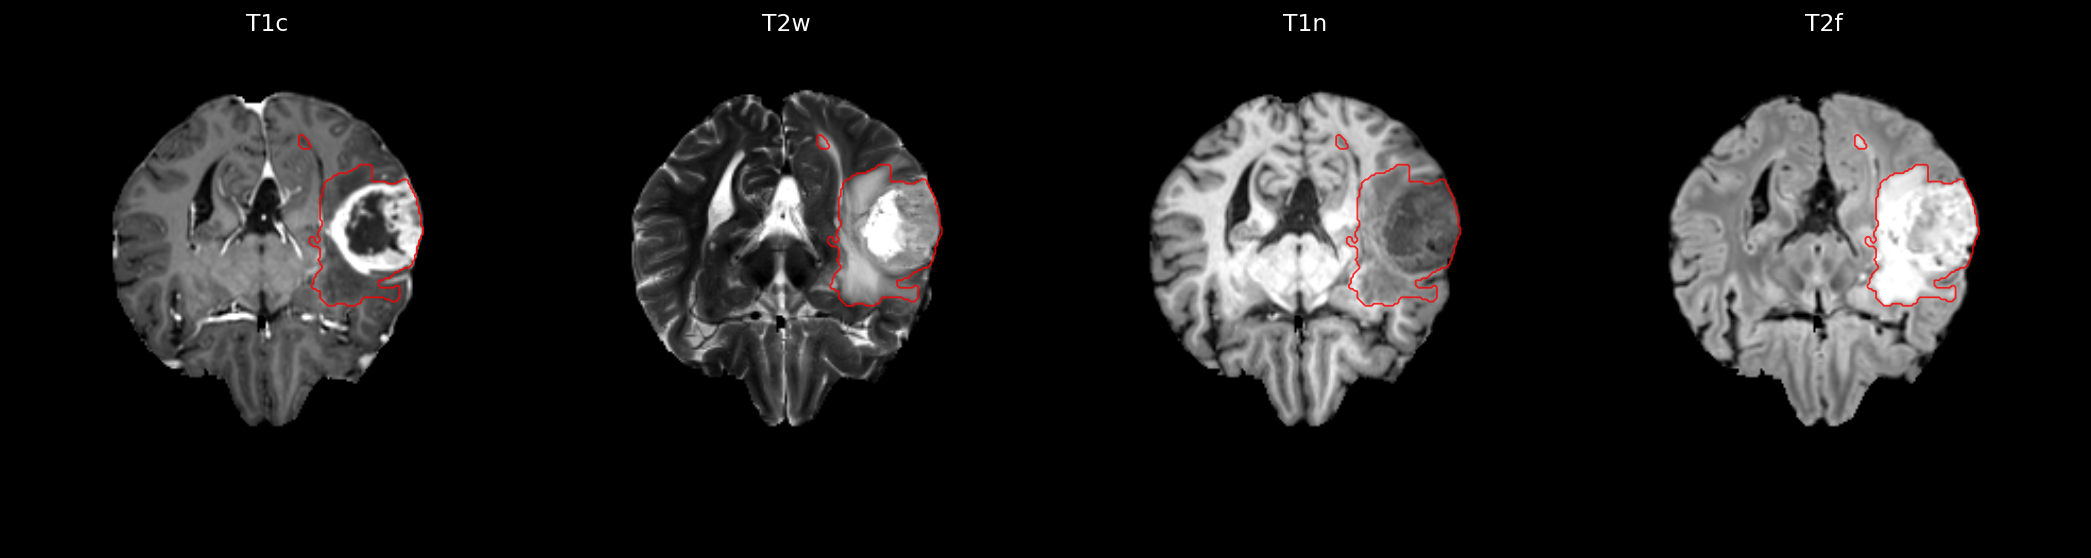
\includegraphics[width=\linewidth]{mri_slices/case_18_mri.png}
\end{center}
{\footnotesize\centering\textit{Red contour = tumor mask. Left to right: T1c, T2w, T1n, T2f (axial slice through tumor center).}\\}

\sectionbar{Proposed Treatment Plans for Next Interval}
{\footnotesize\textit{One option is the actual physician-prescribed regimen; the other is an AI-generated candidate. You do not know which is which.}}

\begin{tcolorbox}[colback=optionA,colframe=optionA!60!black,arc=3pt,title={\textbf{Treatment Option A}},fonttitle=\normalsize\bfseries]
  \begin{itemize}[leftmargin=1.5em,itemsep=1pt,topsep=0pt]
    \item \textbf{Adjuvant}: Temozolomide $\times$6 cycles (q28d)
    \item \textbf{Other}: Optune TTF (continuous)
  \end{itemize}
\end{tcolorbox}

\begin{tcolorbox}[colback=optionB,colframe=optionB!60!black,arc=3pt,title={\textbf{Treatment Option B}},fonttitle=\normalsize\bfseries]
  \begin{itemize}[leftmargin=1.5em,itemsep=1pt,topsep=0pt]
    \item \textbf{Immuno}: Avastin $\times$ongoing cycles (q14d)
    \item \textbf{Other}: optune ttf (continuous)
  \end{itemize}
\end{tcolorbox}

\sectionbar{Expert Judgment (circle or mark ONE)}
\begin{enumerate}[label=\alph*.,leftmargin=2em,itemsep=4pt,topsep=2pt]
  \item[\checkbox] \textbf{Option A} is more clinically reasonable
  \item[\checkbox] \textbf{Option B} is more clinically reasonable
  \item[\checkbox] Both options are \textbf{clinically equivalent} / acceptable
\end{enumerate}

\sectionbar{Confidence Level \normalfont\small(1 = Very uncertain \quad 5 = Very confident)}
\quad $\checkbox$~1 \qquad $\checkbox$~2 \qquad $\checkbox$~3 \qquad $\checkbox$~4 \qquad $\checkbox$~5

\sectionbar{Optional Comment}
\vspace{1.5cm}\hrule\vspace{0.8cm}\hrule

{\footnotesize\textcolor{gray}{\hfill Generated: 2026-05-08 \quad Study ID: CLARITY-BLIND-18}}
\newpage

\begin{tcolorbox}[colback=headerblue,colframe=headerblue,arc=3pt]
  \color{white}\large\bfseries
  Case 19 \hfill TP1 $\rightarrow$ TP2
\end{tcolorbox}
{\footnotesize\textit{Patient identity anonymized. Do not attempt to de-identify.}}

\sectionbar{Patient Summary}
\begin{tabular}{@{}p{5.5cm}p{10cm}@{}}
  \textbf{\small Age / Sex:} & {\small 53 / Male} \\
  \textbf{\small Race:} & {\small White} \\
  \textbf{\small Diagnosis:} & {\small GBM, WHO Grade 4} \\
  \textbf{\small Days from diagnosis:} & {\small 102} \\
  \textbf{\small Disease status:} & {\small Progression documented} \\
  \textbf{\small Key molecular markers:} & {\small IDH1 WT;  IDH2 WT;  MGMT unmethylated} \\
  \textbf{\small Interval to next scan:} & {\small 92 days} \\
\end{tabular}

\sectionbar{Prior Treatment (at pre-scan timepoint)}
\begin{itemize}[leftmargin=1.5em,itemsep=0pt,topsep=2pt]
  \item \textbf{RT}: 60.0\,Gy / 30 fractions
  \item \textbf{Chemo}: Temozolomide (continuous)
  \item \textbf{Brachy}: Gliadel wafer
\end{itemize}

\sectionbar{MRI at Pre-treatment Timepoint}
\begin{center}
  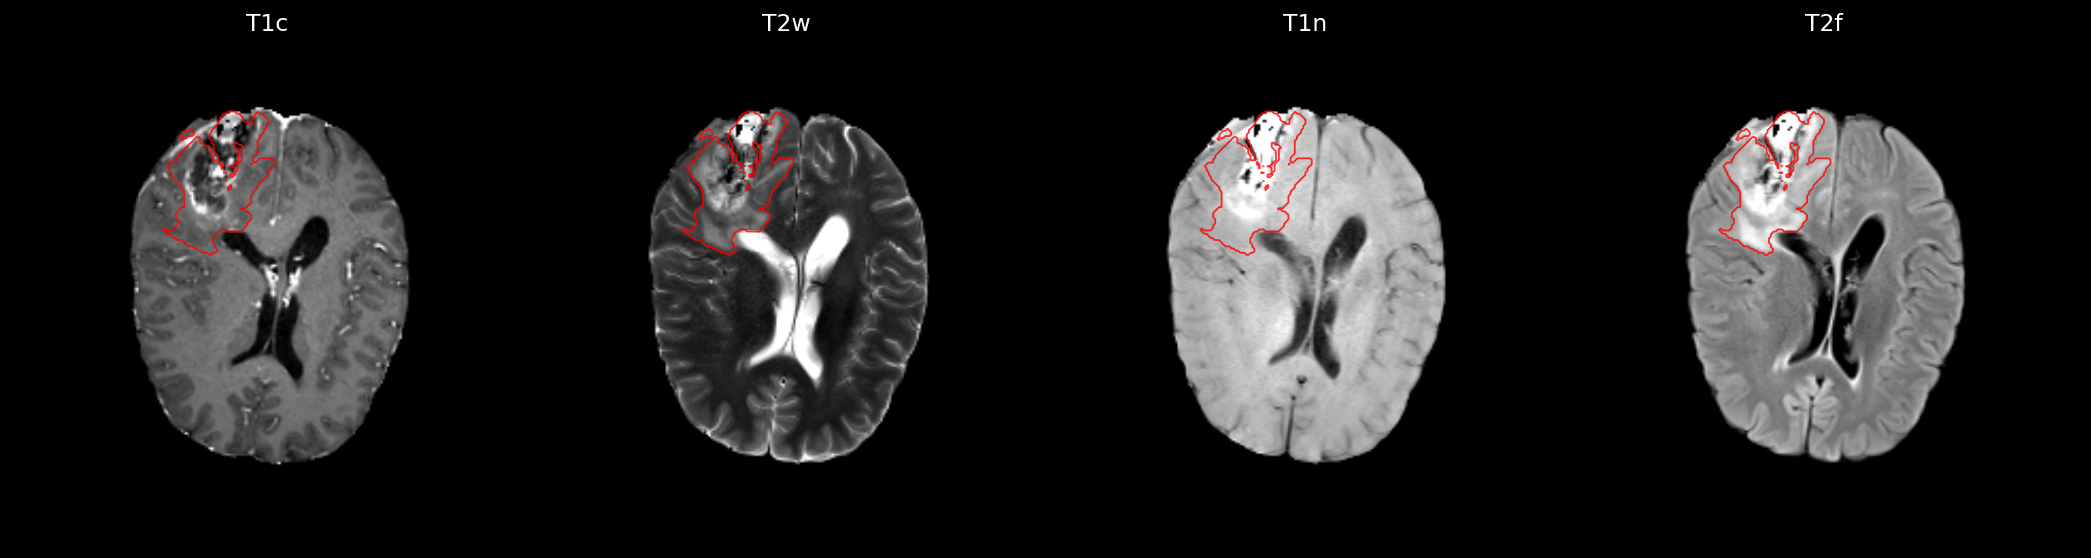
\includegraphics[width=\linewidth]{mri_slices/case_19_mri.png}
\end{center}
{\footnotesize\centering\textit{Red contour = tumor mask. Left to right: T1c, T2w, T1n, T2f (axial slice through tumor center).}\\}

\sectionbar{Proposed Treatment Plans for Next Interval}
{\footnotesize\textit{One option is the actual physician-prescribed regimen; the other is an AI-generated candidate. You do not know which is which.}}

\begin{tcolorbox}[colback=optionA,colframe=optionA!60!black,arc=3pt,title={\textbf{Treatment Option A}},fonttitle=\normalsize\bfseries]
  \begin{itemize}[leftmargin=1.5em,itemsep=1pt,topsep=0pt]
    \item \textbf{Adjuvant}: Temozolomide $\times$6 cycles (q28d)
    \item \textbf{Other}: Optune TTF (continuous)
  \end{itemize}
\end{tcolorbox}

\begin{tcolorbox}[colback=optionB,colframe=optionB!60!black,arc=3pt,title={\textbf{Treatment Option B}},fonttitle=\normalsize\bfseries]
  \begin{itemize}[leftmargin=1.5em,itemsep=1pt,topsep=0pt]
    \item \textbf{Adjuvant}: Temozolomide $\times$7 cycles (q28d)
    \item \textbf{Other}: optune ttf (continuous)
  \end{itemize}
\end{tcolorbox}

\sectionbar{Expert Judgment (circle or mark ONE)}
\begin{enumerate}[label=\alph*.,leftmargin=2em,itemsep=4pt,topsep=2pt]
  \item[\checkbox] \textbf{Option A} is more clinically reasonable
  \item[\checkbox] \textbf{Option B} is more clinically reasonable
  \item[\checkbox] Both options are \textbf{clinically equivalent} / acceptable
\end{enumerate}

\sectionbar{Confidence Level \normalfont\small(1 = Very uncertain \quad 5 = Very confident)}
\quad $\checkbox$~1 \qquad $\checkbox$~2 \qquad $\checkbox$~3 \qquad $\checkbox$~4 \qquad $\checkbox$~5

\sectionbar{Optional Comment}
\vspace{1.5cm}\hrule\vspace{0.8cm}\hrule

{\footnotesize\textcolor{gray}{\hfill Generated: 2026-05-08 \quad Study ID: CLARITY-BLIND-19}}
\newpage

\begin{tcolorbox}[colback=headerblue,colframe=headerblue,arc=3pt]
  \color{white}\large\bfseries
  Case 20 \hfill TP1 $\rightarrow$ TP2
\end{tcolorbox}
{\footnotesize\textit{Patient identity anonymized. Do not attempt to de-identify.}}

\sectionbar{Patient Summary}
\begin{tabular}{@{}p{5.5cm}p{10cm}@{}}
  \textbf{\small Age / Sex:} & {\small 61 / Female} \\
  \textbf{\small Race:} & {\small White} \\
  \textbf{\small Diagnosis:} & {\small GBM, WHO Grade 4} \\
  \textbf{\small Days from diagnosis:} & {\small 129} \\
  \textbf{\small Disease status:} & {\small Progression documented} \\
  \textbf{\small Key molecular markers:} & {\small IDH1 WT;  IDH2 WT;  MGMT unmethylated} \\
  \textbf{\small Interval to next scan:} & {\small 129 days} \\
\end{tabular}

\sectionbar{Prior Treatment (at pre-scan timepoint)}
\begin{itemize}[leftmargin=1.5em,itemsep=0pt,topsep=2pt]
  \item \textbf{RT}: ?\,Gy / ? fractions
  \item \textbf{Chemo}: Temozolomide (continuous)
\end{itemize}

\sectionbar{MRI at Pre-treatment Timepoint}
\begin{center}
  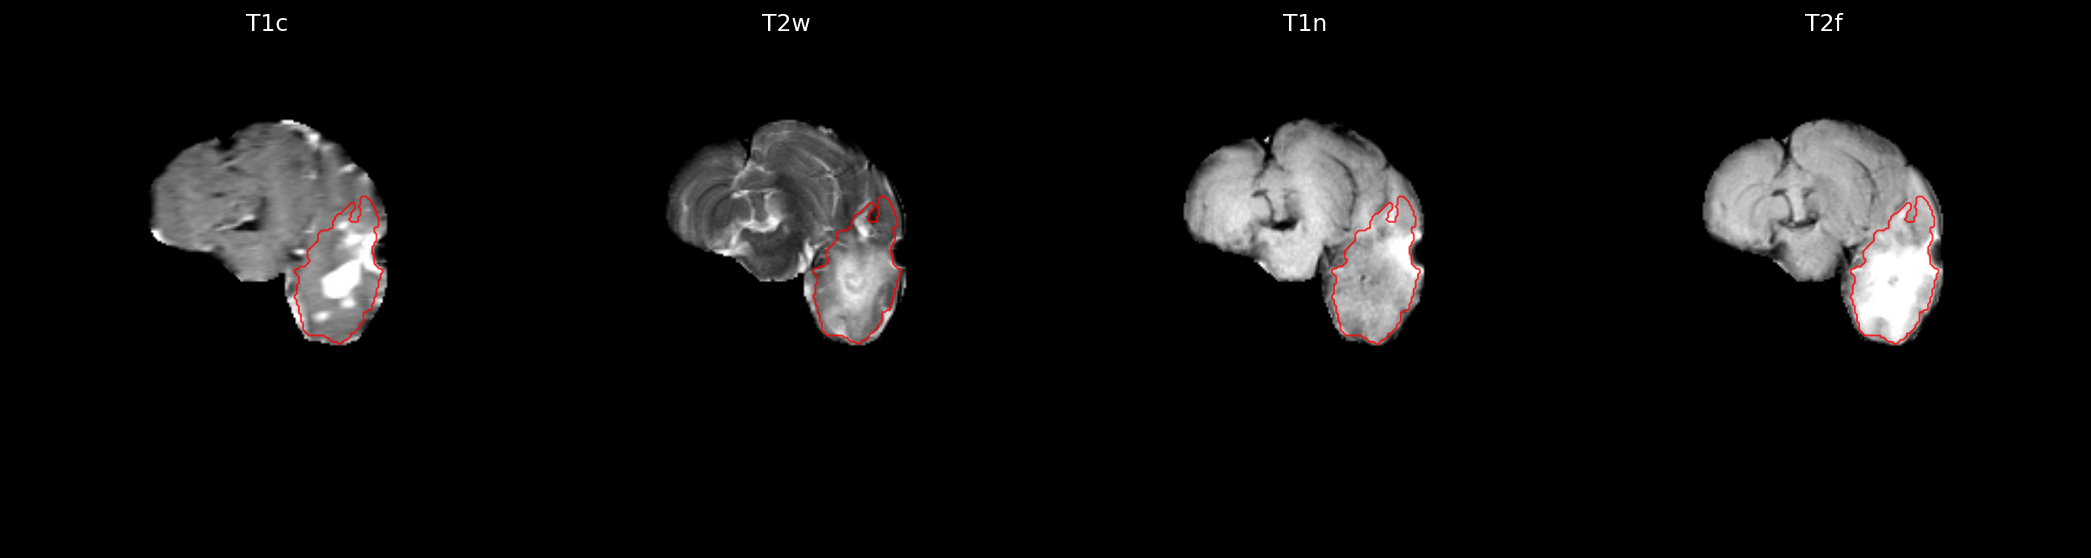
\includegraphics[width=\linewidth]{mri_slices/case_20_mri.png}
\end{center}
{\footnotesize\centering\textit{Red contour = tumor mask. Left to right: T1c, T2w, T1n, T2f (axial slice through tumor center).}\\}

\sectionbar{Proposed Treatment Plans for Next Interval}
{\footnotesize\textit{One option is the actual physician-prescribed regimen; the other is an AI-generated candidate. You do not know which is which.}}

\begin{tcolorbox}[colback=optionA,colframe=optionA!60!black,arc=3pt,title={\textbf{Treatment Option A}},fonttitle=\normalsize\bfseries]
  \begin{itemize}[leftmargin=1.5em,itemsep=1pt,topsep=0pt]
    \item \textbf{RT}: ?\,Gy / ? fractions
    \item \textbf{Chemo}: Temozolomide (continuous)
  \end{itemize}
\end{tcolorbox}

\begin{tcolorbox}[colback=optionB,colframe=optionB!60!black,arc=3pt,title={\textbf{Treatment Option B}},fonttitle=\normalsize\bfseries]
  \begin{itemize}[leftmargin=1.5em,itemsep=1pt,topsep=0pt]
    \item \textbf{Immuno}: Bevacizumab $\times$ongoing cycles (q14d)
    \item \textbf{Other}: Dexamethasone (continuous)
  \end{itemize}
\end{tcolorbox}

\sectionbar{Expert Judgment (circle or mark ONE)}
\begin{enumerate}[label=\alph*.,leftmargin=2em,itemsep=4pt,topsep=2pt]
  \item[\checkbox] \textbf{Option A} is more clinically reasonable
  \item[\checkbox] \textbf{Option B} is more clinically reasonable
  \item[\checkbox] Both options are \textbf{clinically equivalent} / acceptable
\end{enumerate}

\sectionbar{Confidence Level \normalfont\small(1 = Very uncertain \quad 5 = Very confident)}
\quad $\checkbox$~1 \qquad $\checkbox$~2 \qquad $\checkbox$~3 \qquad $\checkbox$~4 \qquad $\checkbox$~5

\sectionbar{Optional Comment}
\vspace{1.5cm}\hrule\vspace{0.8cm}\hrule

{\footnotesize\textcolor{gray}{\hfill Generated: 2026-05-08 \quad Study ID: CLARITY-BLIND-20}}
\end{document}